
\documentclass[xcolor=dvipsnames]{beamer}  % for hardcopy add 'trans'

\mode<presentation>
{
  \usetheme{Singapore}
  % or ...
  \setbeamercovered{transparent}
  % or whatever (possibly just delete it)
}

\usefonttheme{professionalfonts}
%\usepackage[english]{babel}
% or whatever
%\usepackage[latin1]{inputenc}
% or whatever
%\usepackage{times}
%\usepackage[T1]{fontenc}
% Or whatever. Note that the encoding and the font should match. If T1
% does not look nice, try deleting the line with the fontenc.

%%%%%%%%%%%%%%%%%%%%%% start my preamble %%%%%%%%%%%%%%%%%%%%%%


\addtobeamertemplate{navigation symbols}{}{%
    \usebeamerfont{footline}%
    \usebeamercolor[fg]{footline}%
    \hspace{1em}%
    \insertframenumber/\inserttotalframenumber
}

\setbeamercolor{footline}{fg=blue}
\setbeamerfont{footline}{series=\bfseries}


%\usepackage{epsfig}
\usepackage{graphicx}
\usepackage{amsmath, amssymb, amsthm}

\usepackage{fancyvrb}

\usepackage{tikz}
\usetikzlibrary{arrows}
\usetikzlibrary{calc}
\usetikzlibrary{intersections}
\usetikzlibrary{decorations}
\usepackage{pgf}
\usepackage{pgfplots}
\pgfplotsset{compat=1.13}

\usepackage{graphviz}
 
\usepackage{verbatim}


\usepackage{algorithmicx,algpseudocode}


%font
\usepackage{mathpazo}
%\usepackage[usenames, dvipsnames]{color}

%\usepackage[linesnumbered, ruled, lined]{algorithm2e}

\usepackage{xr}
\externaldocument[ET-]{et}


\newcommand*{\theorembreak}{\usebeamertemplate{theorem end}\framebreak\usebeamertemplate{theorem begin}}

\newcommand{\newtopic}[1]{\textcolor{Green}{\Large \bf #1}}
\newcommand{\navy}[1]{\textcolor{Blue}{\bf #1}}
\newcommand{\navymth}[1]{\textcolor{Blue}{#1}}
\newcommand{\red}[1]{\textcolor{red}{#1}}


\definecolor{pale}{RGB}{235, 235, 235}
\definecolor{pale2}{RGB}{175,238,238}
\definecolor{turquois4}{RGB}{0,134,139}

% Typesetting code
\definecolor{bg}{rgb}{0.95,0.95,0.95}
\usepackage{minted}
\usemintedstyle{friendly}
\newminted{python}{mathescape,frame=lines,framesep=4mm,bgcolor=bg}
\newminted{ipython}{mathescape,frame=lines,framesep=4mm,bgcolor=bg}
\newminted{julia}{mathescape,frame=lines,framesep=4mm,bgcolor=bg}
\newminted{c}{mathescape,linenos=true}
\newminted{r}{mathescape,  frame=none, baselinestretch=1, framesep=2mm}
\renewcommand{\theFancyVerbLine}{\sffamily
    \textcolor[rgb]{0.5,0.5,1.0}{\scriptsize {\arabic{FancyVerbLine}}}}


\usepackage{stmaryrd}

\newcommand{\Fact}{\textcolor{Brown}{\bf Fact. }}
\newcommand{\Facts}{\textcolor{Brown}{\bf Facts }}
\newcommand{\keya}{\textcolor{turquois4}{\bf Key Idea. }}
\newcommand{\Factnodot}{\textcolor{Brown}{\bf Fact }}
\newcommand{\Eg}{\textcolor{ForestGreen}{Example. }}
\newcommand{\Egs}{\textcolor{ForestGreen}{Examples. }}
\newcommand{\Ex}{{\bf Ex. }}
\newcommand{\Thm}{\textcolor{Brown}{\bf Theorem. }}
\newcommand{\Prf}{\textcolor{turquois4}{\bf Proof.}}
\newcommand{\Ass}{\textcolor{turquois4}{\bf Assumption.}} 
\newcommand{\Lem}{\textcolor{Brown}{\bf Lemma. }}

%source code 



% caligraphic
\usepackage{mathrsfs}
\usepackage{bbm}
\usepackage{subfigure}

\newcommand{\argmax}{\operatornamewithlimits{argmax}}
\newcommand{\argmin}{\operatornamewithlimits{argmin}}

\newcommand\T{{\mathpalette\raiseT\intercal}}
\newcommand\raiseT[2]{\raisebox{0.25ex}{$#1#2$}}

\DeclareMathOperator{\cl}{cl}
%\DeclareMathOperator{\argmax}{argmax}
\DeclareMathOperator{\interior}{int}
\DeclareMathOperator{\Prob}{Prob}
\DeclareMathOperator{\kernel}{ker}
\DeclareMathOperator{\diag}{diag}
\DeclareMathOperator{\sgn}{sgn}
\DeclareMathOperator{\determinant}{det}
\DeclareMathOperator{\trace}{trace}
\DeclareMathOperator{\Span}{span}
\DeclareMathOperator{\rank}{rank}
\DeclareMathOperator{\cov}{cov}
\DeclareMathOperator{\corr}{corr}
\DeclareMathOperator{\range}{rng}
\DeclareMathOperator{\var}{var}
\DeclareMathOperator{\mse}{mse}
\DeclareMathOperator{\se}{se}
\DeclareMathOperator{\row}{row}
\DeclareMathOperator{\col}{col}
\DeclareMathOperator{\dimension}{dim}
\DeclareMathOperator{\fracpart}{frac}
\DeclareMathOperator{\proj}{proj}
\DeclareMathOperator{\colspace}{colspace}

\providecommand{\inner}[1]{\left\langle{#1}\right\rangle}

% mics short cuts and symbols
% mics short cuts and symbols
\newcommand{\st}{\ensuremath{\ \mathrm{s.t.}\ }}
\newcommand{\setntn}[2]{ \{ #1 : #2 \} }
\newcommand{\cf}[1]{ \lstinline|#1| }
\newcommand{\otms}[1]{ \leftidx{^\circ}{#1}}

\newcommand{\fore}{\therefore \quad}
\newcommand{\tod}{\stackrel { d } {\to} }
\newcommand{\tow}{\stackrel { w } {\to} }
\newcommand{\toprob}{\stackrel { p } {\to} }
\newcommand{\toms}{\stackrel { ms } {\to} }
\newcommand{\eqdist}{\stackrel {\textrm{ \scriptsize{d} }} {=} }
\newcommand{\iidsim}{\stackrel {\textrm{ {\sc iid }}} {\sim} }
\newcommand{\1}{\mathbbm 1}
\newcommand{\dee}{\,{\rm d}}
\newcommand{\given}{\, | \,}
\newcommand{\la}{\langle}
\newcommand{\ra}{\rangle}

\renewcommand{\rho}{\varrho}

\newcommand{\htau}{ \hat \tau }
\newcommand{\hgamma}{ \hat \gamma }

\newcommand{\boldx}{ {\mathbf x} }
\newcommand{\boldu}{ {\mathbf u} }
\newcommand{\boldv}{ {\mathbf v} }
\newcommand{\boldw}{ {\mathbf w} }
\newcommand{\boldy}{ {\mathbf y} }
\newcommand{\boldb}{ {\mathbf b} }
\newcommand{\bolda}{ {\mathbf a} }
\newcommand{\boldc}{ {\mathbf c} }
\newcommand{\boldi}{ {\mathbf i} }
\newcommand{\bolde}{ {\mathbf e} }
\newcommand{\boldp}{ {\mathbf p} }
\newcommand{\boldq}{ {\mathbf q} }
\newcommand{\bolds}{ {\mathbf s} }
\newcommand{\boldt}{ {\mathbf t} }
\newcommand{\boldz}{ {\mathbf z} }

\newcommand{\boldzero}{ {\mathbf 0} }
\newcommand{\boldone}{ {\mathbf 1} }

\newcommand{\boldalpha}{ {\boldsymbol \alpha} }
\newcommand{\boldbeta}{ {\boldsymbol \beta} }
\newcommand{\boldgamma}{ {\boldsymbol \gamma} }
\newcommand{\boldtheta}{ {\boldsymbol \theta} }
\newcommand{\boldxi}{ {\boldsymbol \xi} }
\newcommand{\boldtau}{ {\boldsymbol \tau} }
\newcommand{\boldepsilon}{ {\boldsymbol \epsilon} }
\newcommand{\boldmu}{ {\boldsymbol \mu} }
\newcommand{\boldSigma}{ {\boldsymbol \Sigma} }
\newcommand{\boldOmega}{ {\boldsymbol \Omega} }
\newcommand{\boldPhi}{ {\boldsymbol \Phi} }
\newcommand{\boldLambda}{ {\boldsymbol \Lambda} }
\newcommand{\boldphi}{ {\boldsymbol \phi} }

\newcommand{\Sigmax}{ {\boldsymbol \Sigma_{\boldx}}}
\newcommand{\Sigmau}{ {\boldsymbol \Sigma_{\boldu}}}
\newcommand{\Sigmaxinv}{ {\boldsymbol \Sigma_{\boldx}^{-1}}}
\newcommand{\Sigmav}{ {\boldsymbol \Sigma_{\boldv \boldv}}}

\newcommand{\hboldx}{ \hat {\mathbf x} }
\newcommand{\hboldy}{ \hat {\mathbf y} }
\newcommand{\hboldb}{ \hat {\mathbf b} }
\newcommand{\hboldu}{ \hat {\mathbf u} }
\newcommand{\hboldtheta}{ \hat {\boldsymbol \theta} }
\newcommand{\hboldtau}{ \hat {\boldsymbol \tau} }
\newcommand{\hboldmu}{ \hat {\boldsymbol \mu} }
\newcommand{\hboldbeta}{ \hat {\boldsymbol \beta} }
\newcommand{\hboldgamma}{ \hat {\boldsymbol \gamma} }
\newcommand{\hboldSigma}{ \hat {\boldsymbol \Sigma} }

\newcommand{\boldA}{\mathbf A}
\newcommand{\boldB}{\mathbf B}
\newcommand{\boldC}{\mathbf C}
\newcommand{\boldD}{\mathbf D}
\newcommand{\boldI}{\mathbf I}
\newcommand{\boldL}{\mathbf L}
\newcommand{\boldM}{\mathbf M}
\newcommand{\boldP}{\mathbf P}
\newcommand{\boldQ}{\mathbf Q}
\newcommand{\boldR}{\mathbf R}
\newcommand{\boldX}{\mathbf X}
\newcommand{\boldU}{\mathbf U}
\newcommand{\boldV}{\mathbf V}
\newcommand{\boldW}{\mathbf W}
\newcommand{\boldY}{\mathbf Y}
\newcommand{\boldZ}{\mathbf Z}

\newcommand{\bSigmaX}{ {\boldsymbol \Sigma_{\hboldbeta}} }
\newcommand{\hbSigmaX}{ \mathbf{\hat \Sigma_{\hboldbeta}} }

\newcommand{\RR}{\mathbbm R}
\newcommand{\CC}{\mathbbm C}
\newcommand{\NN}{\mathbbm N}
\newcommand{\PP}{\mathbbm P}
\newcommand{\EE}{\mathbbm E \nobreak\hspace{.1em}}
\newcommand{\EEP}{\mathbbm E_P \nobreak\hspace{.1em}}
\newcommand{\ZZ}{\mathbbm Z}
\newcommand{\QQ}{\mathbbm Q}


\newcommand{\XX}{\mathcal X}

\newcommand{\aA}{\mathcal A}
\newcommand{\fF}{\mathscr F}
\newcommand{\bB}{\mathscr B}
\newcommand{\iI}{\mathscr I}
\newcommand{\rR}{\mathscr R}
\newcommand{\dD}{\mathcal D}
\newcommand{\lL}{\mathcal L}
\newcommand{\llL}{\mathcal{H}_{\ell}}
\newcommand{\gG}{\mathcal G}
\newcommand{\hH}{\mathcal H}
\newcommand{\nN}{\textrm{\sc n}}
\newcommand{\lN}{\textrm{\sc ln}}
\newcommand{\pP}{\mathscr P}
\newcommand{\qQ}{\mathscr Q}
\newcommand{\xX}{\mathcal X}

\newcommand{\ddD}{\mathscr D}


\newcommand{\R}{{\texttt R}}
\newcommand{\risk}{\mathcal R}
\newcommand{\Remp}{R_{{\rm emp}}}

\newcommand*\diff{\mathop{}\!\mathrm{d}}
\newcommand{\ess}{ \textrm{{\sc ess}} }
\newcommand{\tss}{ \textrm{{\sc tss}} }
\newcommand{\rss}{ \textrm{{\sc rss}} }
\newcommand{\rssr}{ \textrm{{\sc rssr}} }
\newcommand{\ussr}{ \textrm{{\sc ussr}} }
\newcommand{\zdata}{\mathbf{z}_{\mathcal D}}
\newcommand{\Pdata}{P_{\mathcal D}}
\newcommand{\Pdatatheta}{P^{\mathcal D}_{\theta}}
\newcommand{\Zdata}{Z_{\mathcal D}}




\newcommand{\e}[1]{\mathbbm{E}[{#1}]}
\newcommand{\p}[1]{\mathbbm{P}({#1})}

%\theoremstyle{plain}
%\newtheorem{axiom}{Axiom}[section]
%\newtheorem{theorem}{Theorem}[section]
%\newtheorem{corollary}{Corollary}[section]
%\newtheorem{lemma}{Lemma}[section]
%\newtheorem{proposition}{Proposition}[section]
%
%\theoremstyle{definition}
%\newtheorem{definition}{Definition}[section]
%\newtheorem{example}{Example}[section]
%\newtheorem{remark}{Remark}[section]
%\newtheorem{notation}{Notation}[section]
%\newtheorem{assumption}{Assumption}[section]
%\newtheorem{condition}{Condition}[section]
%\newtheorem{exercise}{Ex.}[section]
%\newtheorem{fact}{Fact}[section]

% Bibliography
\usepackage[authordate,uniquename=false,firstinits,backend=biber,maxcitenames=2]{biblatex-chicago}
\DeclareFieldFormat[article]{title}{#1}
\DeclareFieldFormat[inproceedings]{title}{#1}
\addbibresource{et_newbib.bib}
\renewcommand{\cite}{\textcite}



\setlength{\parskip}{1.5ex plus0.5ex minus0.5ex}


\setlength{\jot}{12pt} 







\title{A Primer in Econometric Theory}

\subtitle
{Lecture 1: Vector Spaces}


\author{John Stachurski \\ \tiny Lectures by Akshay Shanker}

\begin{document}

\begin{frame}
  \titlepage
\end{frame}


\begin{frame}

    \frametitle{Overview}

    \vspace{2em}
    Linear algebra is an important foundation for mathematics and, in particular, for Econometrics: 
    
    \begin{itemize}
        \item performing basic arithmetic on data 
        \item solving linear equations using data
        \item advanced operations such as quadratic minimisation 
    \end{itemize}
    
    \vspace{1em}
    Focus of this chapter:
    \begin{enumerate}
        \item vector spaces: linear operations, norms, linear subspaces, 
        linear independence, bases, etc.
        \item orthogonal projection theorem 
    \end{enumerate}
 
\end{frame}

\section{Vector Space}

\begin{frame}
    \frametitle{Vector Space}
    
    \vspace{2em}
    The symbol $\RR^N$ represents set of all vectors of length $N$, or $N$ vectors 

    \vspace{.7em}

    An $N$-vector $\boldx$ is a tuple of $N$ real numbers:
    $$
    \boldx = (x_1, \ldots, x_N)
        \quad
        \text{ where } 
        \quad x_n \in \RR \text{ for each } n
    $$  
    \vspace{1em}
    We can also write $\boldx$ vertically, like so: 
    %
    \begin{equation*}
        \boldx = 
        \left(
        \begin{array}{c}
            x_1 \\
            x_2 \\
            \vdots \\
            x_N
        \end{array}
        \right)
    \end{equation*}
    
\end{frame}

%\begin{frame}
    
%    \begin{figure}
%       \begin{center}
%        \scalebox{.95}{\input{../tikzfigs/vec.tex}}
%        \caption{\label{f:vec} Visualization of vector $\boldx$ in $\RR^2$}
%       \end{center}
%    \end{figure}

%\end{frame}


\begin{frame}

    \begin{figure}
       \begin{center}
        \scalebox{.4}{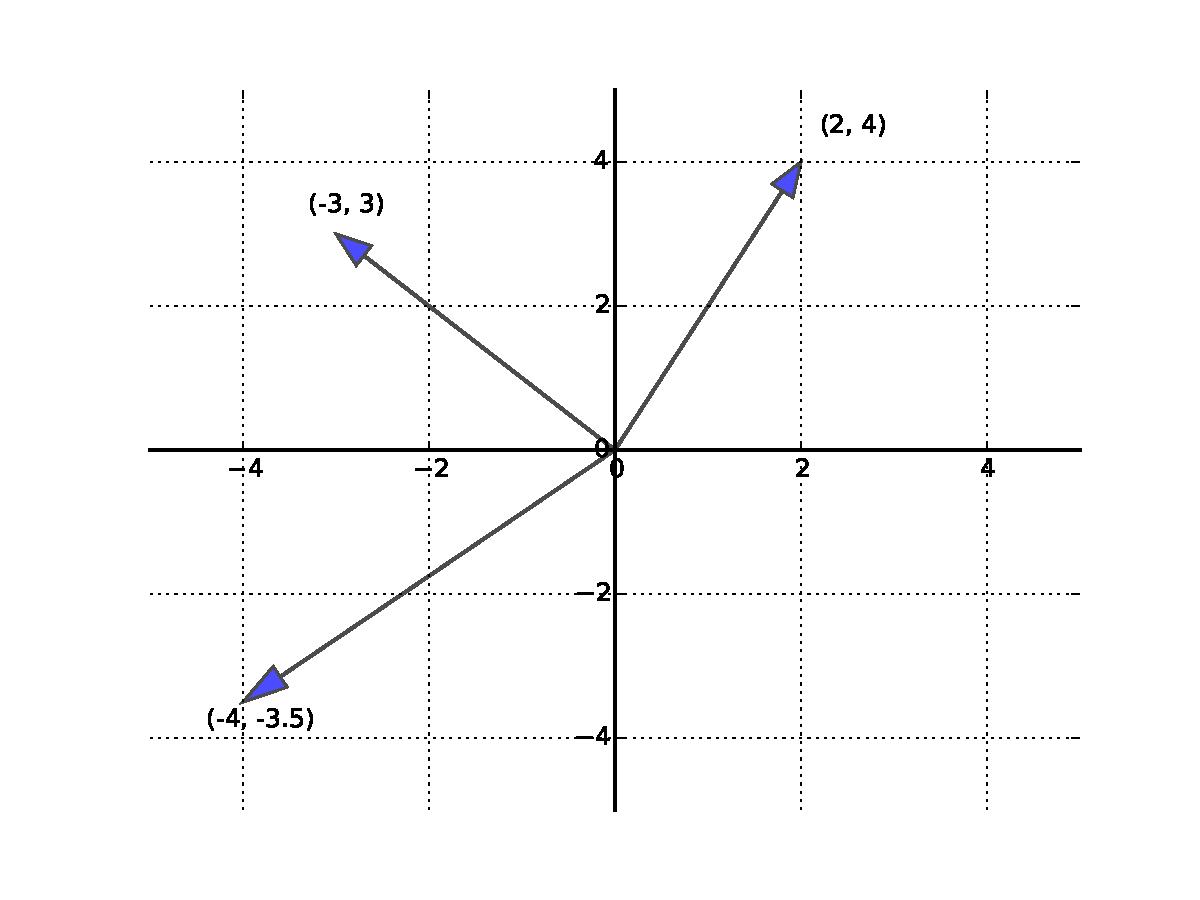
\includegraphics{vecs.pdf}}
        \caption{Three vectors in $\RR^2$ }
       \end{center}
    \end{figure}

\end{frame}


\begin{frame}

    \vspace{2em}
    The vector of ones will be denoted $\boldone$ 
    
    %
    \begin{equation*}
        \boldone := 
        \left(
        \begin{array}{c}
            1 \\
            \vdots \\
            1
        \end{array}
        \right)
    \end{equation*}
    %

    Vector of zeros will be denoted $\boldzero$

    %
    \begin{equation*}
        \boldzero := 
        \left(
        \begin{array}{c}
            0 \\
            \vdots \\
            0
        \end{array}
        \right)
    \end{equation*}

\end{frame}


\begin{frame}
    \frametitle{Linear Operations}

    \vspace{2em}
    
    Two fundamental algebraic operations: 
    %
    \begin{enumerate}
        \item Vector addition 
        \item Scalar multiplication
    \end{enumerate}
    
    
    1. \navy{Sum} of $\boldx \in \RR^N$ and $\boldy \in \RR^N$ defined by
    
    \begin{equation*}
        \boldx + \boldy 
        :=: 
        \left(
        \begin{array}{c}
            x_1 \\
            x_2 \\
            \vdots \\
            x_N
        \end{array}
        \right)
        +
        \left(
        \begin{array}{c}
             y_1 \\
             y_2 \\
            \vdots \\
             y_N
        \end{array}
        \right)
        :=
        \left(
        \begin{array}{c}
            x_1 + y_1 \\
            x_2 + y_2 \\
            \vdots \\
            x_N + y_N
        \end{array}
        \right)
    \end{equation*}
    %


\end{frame}


\begin{frame}

    Example 1:

    \begin{equation*}
        \left(
        \begin{array}{c}
            1 \\
            2 \\
            3 \\
            4
        \end{array}
        \right)
        +
        \left(
        \begin{array}{c}
             2 \\
             4 \\
             6 \\
             8
        \end{array}
        \right)
        :=
        \left(
        \begin{array}{c}
            3 \\
            6 \\
            9 \\
            12
        \end{array}
        \right)
    \end{equation*}
    %

    Example 2:

    \begin{equation*}
        \left(
        \begin{array}{c}
            1 \\
            2 \\
            3 \\
            4
        \end{array}
        \right)
        +
        \left(
        \begin{array}{c}
             1 \\
             1 \\
             1 \\
             1
        \end{array}
        \right)
        :=
        \left(
        \begin{array}{c}
            2 \\
            3 \\
            4 \\
            5
        \end{array}
        \right)
    \end{equation*}
    
\end{frame}

\begin{frame}
    

\begin{figure}

  \begin{center}
    \scalebox{.4}{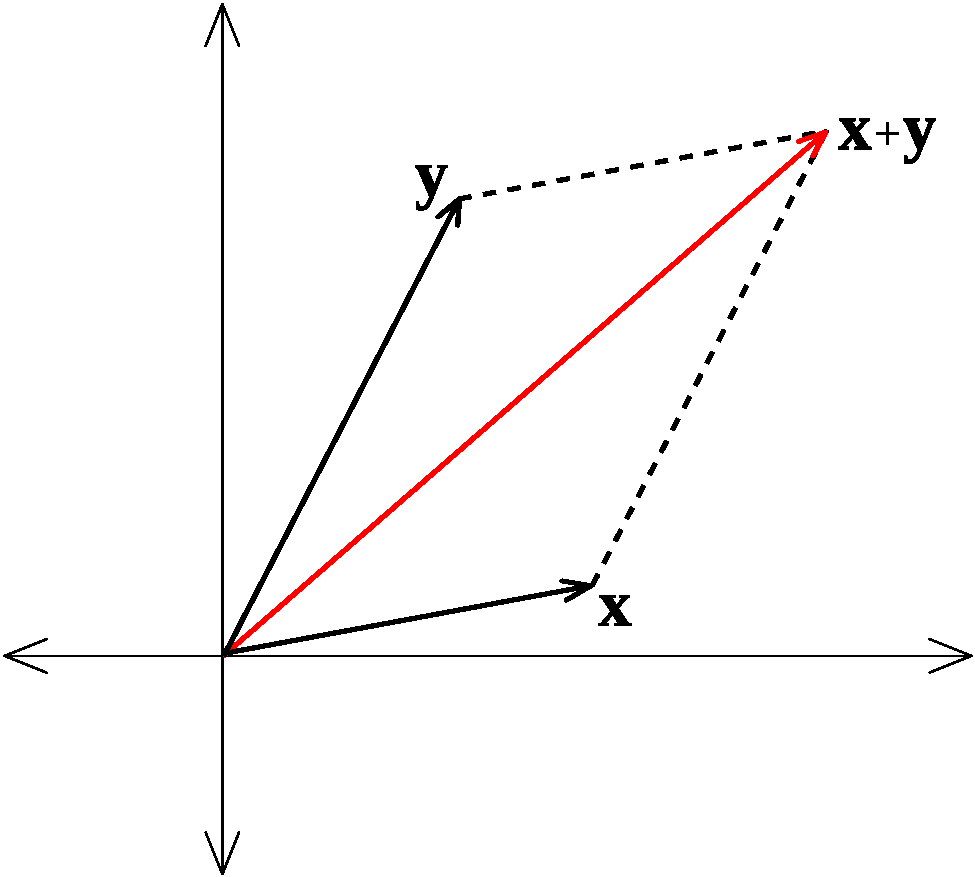
\includegraphics{vec_add.pdf}}
   \caption{\label{f:vec_add} Vector addition}
  \end{center}
  
\end{figure}



\end{frame}


\begin{frame}
    
    2. \navy{Scalar product} of $\alpha \in \RR$ and $\boldx \in \RR^N$ defined by
    
    \begin{equation*}
        \alpha \boldx 
        =
        \alpha \left(
        \begin{array}{c}
            x_1 \\
            x_2 \\
            \vdots \\
            x_N
        \end{array}
        \right)
        :=
        \left(
        \begin{array}{c}
            \alpha x_1 \\
            \alpha x_2 \\
            \vdots \\
            \alpha x_N
        \end{array}
        \right)
    \end{equation*}
    %

\end{frame}



\begin{frame}

    Example 1:

    \begin{equation*}
        0.5 
        \left(
        \begin{array}{c}
            1 \\
            2 \\
            3 \\
            4
        \end{array}
        \right)
        :=
        \left(
        \begin{array}{c}
            0.5 \\
            1.0 \\
            1.5 \\
            2.0 
        \end{array}
        \right)
    \end{equation*}
    %

    Example 2:

    \begin{equation*}
        -1
        \left(
        \begin{array}{c}
            1 \\
            2 \\
            3 \\
            4
        \end{array}
        \right)
        :=
        \left(
        \begin{array}{c}
            -1 \\
            -2 \\
            -3 \\
            -4
        \end{array}
        \right)
    \end{equation*}
    %
\end{frame}

\begin{frame}
    
\begin{figure}
  \begin{center}
   \scalebox{.4}{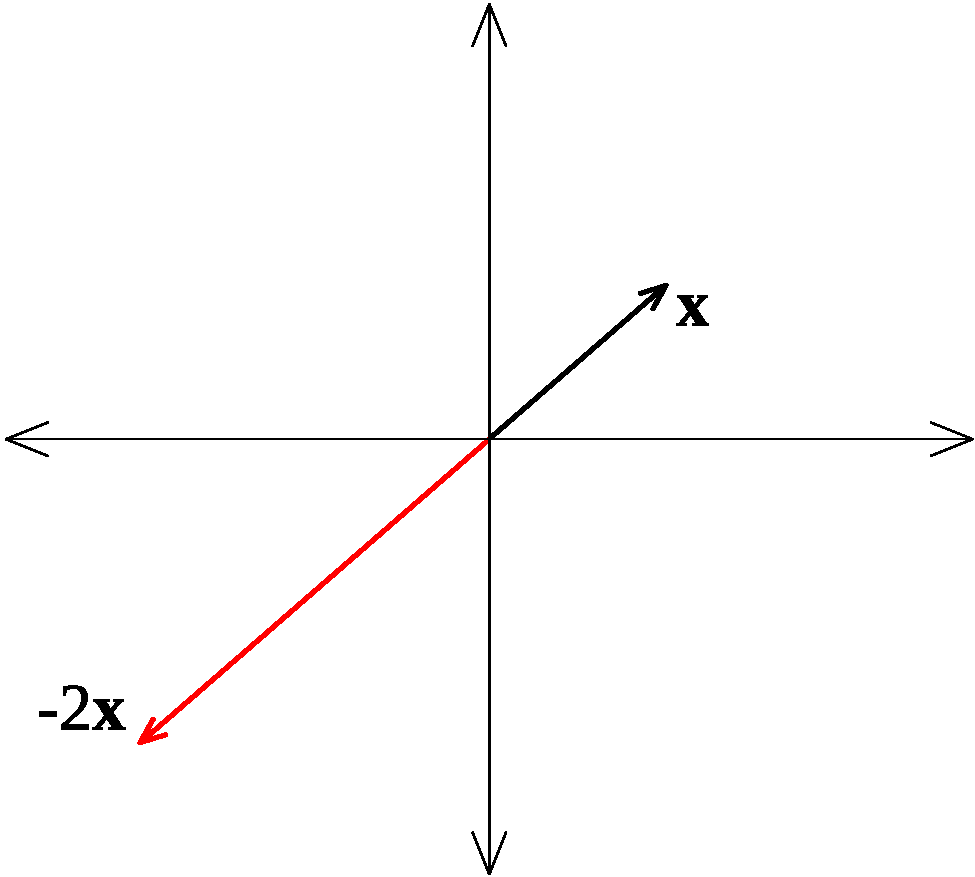
\includegraphics{vec_scalar.pdf}}
    \caption{\label{f:vec_scalar} Scalar multiplication}
 \end{center}
\end{figure}

\end{frame}



\begin{frame}
    
    \vspace{2em}
    Subtraction performed element by element, analogous to addition 

    \begin{equation*}
        \boldx - \boldy 
        :=
        \left(
        \begin{array}{c}
            x_1 - y_1 \\
            x_2 - y_2 \\
            \vdots \\
            x_N - y_N
        \end{array}
        \right)
    \end{equation*}
    
    \vspace{.7em}
    Definition can be given in terms of addition and scalar multiplication

    \begin{equation*}
      \boldx - \boldy := \boldx + (-1) \boldy      
    \end{equation*}

\end{frame}



\begin{frame}

     \vspace{2em}
    \begin{figure}
       \begin{center}
        \scalebox{.375}{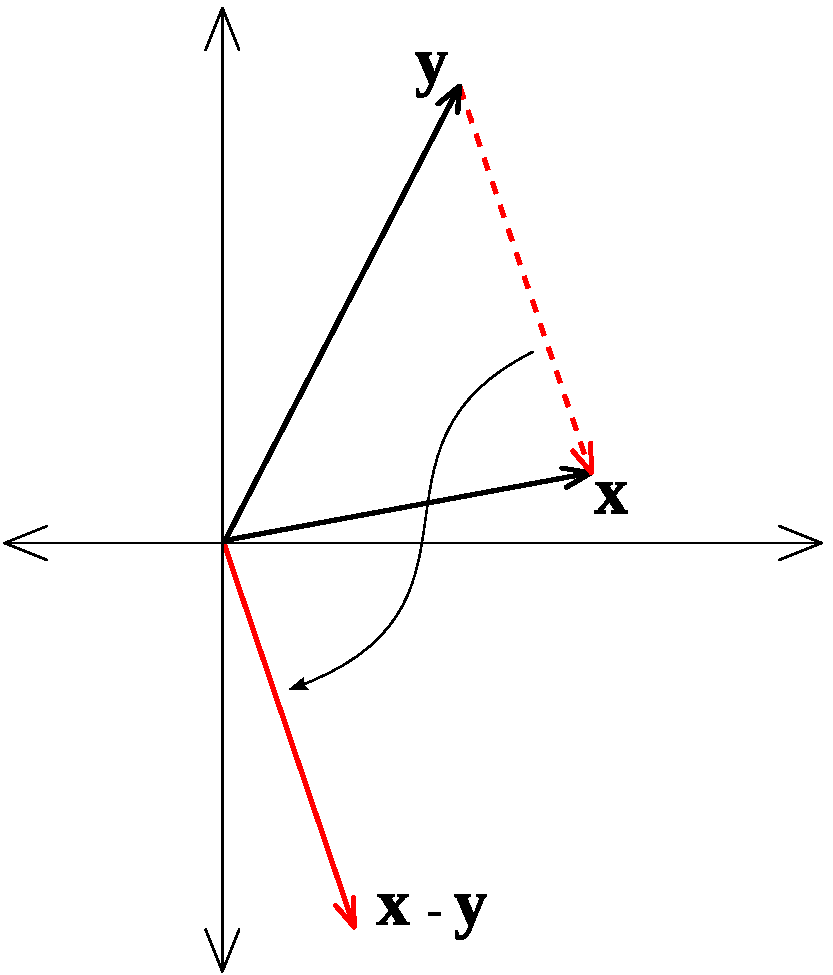
\includegraphics{vec_minus.pdf}}
       \caption{\label{f:vec_minus} Difference between vectors}
       \end{center}
    \end{figure}

\end{frame}




%begin{frame}[fragile]
    
%    Incidentally, most high level numerical libraries treat vector addition
%    and scalar multiplication in the same way --- elementwise

%\begin{pythoncode}
%    In [1]: import numpy as np

%    In [2]: x = np.array((2, 4, 6))

%    In [3]: y = np.array((10, 10, 10))

%    In [4]: x + y  # Vector addition
%    Out[4]: array([12, 14, 16])

%    In [6]: 2 * x  # Scalar multiplication
%    Out[6]: array([ 4,  8, 12])
%\end{pythoncode}


%\end{frame}

\begin{frame}
    \frametitle{Inner Product}
    
     \vspace{2em}
    The \navy{inner product} of two vectors $\boldx$ and $\boldy$ in $\RR^N$ is
    denoted by $\inner{\boldx,  \boldy}$, and defined
    as the sum of the products of their elements:
    
    \vspace{.7em}
    \begin{equation*}
        \label{eq:dipv}
        \inner{\boldx,  \boldy} := \sum_{n=1}^N x_n y_n 
    \end{equation*}
    
    
\end{frame}


%\begin{frame}[fragile]


%    \begin{pythoncode}
%In [1]: import numpy as np

%In [2]: x = np.array((1, 2, 3, 4))

%In [3]: y = np.array((2, 4, 6, 8))

%In [6]: np.sum(x * y)  # Inner product
%Out[6]: 60
%    \end{pythoncode}
    
%\end{frame}

\begin{frame}

    \vspace{2em}
    \Fact \eqref{ET-fa:profno}
    
    For any $\alpha, \beta \in \RR$ and any $\boldx, \boldy \in \RR^N$, the following 
    statements are true:
    %
    \begin{enumerate}
        \item $\inner{\boldx, \boldy} = \inner{\boldy, \boldx}$,
        \item $\inner{\alpha \boldx, \beta \boldy} =  \alpha \beta
            \inner{\boldx, \boldy}$, and
        \item $\inner{\boldx, \alpha \boldy + \beta \boldz} =  \alpha
            \inner{\boldx, \boldy} + \beta \inner{\boldx, \boldz}$.
    \end{enumerate}
    
    \vspace{1em}
    Properties easy to check using definitions of scalar multiplication and inner product

    For example, to show 2.,
    pick any $\alpha, \beta \in \RR$ and any $\boldx, \boldy \in
    \RR^N$:
    %
    \begin{equation*}
        \inner{\alpha \boldx, \beta \boldy}
        = \sum_{n=1}^N \alpha x_n \beta y_n
        = \alpha \beta \sum_{n=1}^N x_n y_n 
        = \alpha \beta \inner{\boldx, \boldy}
    \end{equation*}

\end{frame}

\begin{frame}
    \frametitle{Norms and Distance}
    
     \vspace{2em}
    The (Euclidean) \navy{norm} of $\boldx \in \RR^N$ is defined as
    %
    \begin{equation*}
        \label{eq:eucnorm}
        \| \boldx \| := \sqrt{\inner{\boldx, \boldx}} 
    \end{equation*}
    %
    
    \vspace{.7em}
    Interpretation:
    %
    \begin{itemize}
        \item $\| \boldx \|$ represents the ``length'' of $\boldx$
            \vspace{0.5em}
        \item $\| \boldx - \boldy \|$ represents distance between $\boldx$ and $\boldy$
    \end{itemize}

\end{frame}

%\begin{frame}
    
%    \begin{figure}
%       \begin{center}
%           \scalebox{.95}{\input{../tikzfigs/vec.tex}}
%        \caption{\label{f:vec_rpt} Length of red line $= \sqrt{x_1^2 + x_2^2}
%            =: \|\boldx\|$ }
%       \end{center}
%    \end{figure}

%\end{frame}

\begin{frame}
    
    \vspace{2em}
    \Fact\eqref{ET-fa:profno} For any $\alpha \in \RR$ and any $\boldx, \boldy \in \RR^N$,
    the following 
    statements are true:
    %
    \begin{enumerate}
        \item $\| \boldx \| \geq 0$ and $\| \boldx \| = 0$ if and only if
            $\boldx = \boldzero$
            \vspace{1em}
        \item $\| \alpha \boldx \| = |\alpha| \| \boldx \|$
            \vspace{1em}
        \item $\| \boldx + \boldy \| \leq  \| \boldx \| + \| \boldy \|$
            (\navy{triangle inequality})
            \vspace{1em}
        \item $| \boldx' \boldy | \leq  \| \boldx \| \| \boldy \|$
            (\navy{Cauchy-Schwarz inequality})
    \end{enumerate}
    %

\end{frame}

\begin{frame}

    \vspace{2em}
    Properties 1. and 2. are straight-forward to prove (exercise)
    
    Property 4. is addressed in ET exercise \ref{ET-ex:pcsin}
    
    \vspace{.7em}
    To show property 3, by properties of the inner product in fact \ref{ET-fa:innpp}
    %
    \begin{align*}
        \label{eq:tifcs}
         \| \boldx + \boldy \|^2
        & = \inner{\boldx + \boldy, \boldx + \boldy}
        \\& = \inner{\boldx, \boldx} + 2 \inner{\boldx, \boldy} +  \inner{\boldy,
        \boldy}
        \\& \leq \inner{\boldx, \boldx} + 2 | \! \inner{\boldx, \boldy} \! | +  \inner{\boldy,
        \boldy}
    \end{align*}
    %
\end{frame}

\begin{frame}
    
     \vspace{2em}
    Apply the Cauchy--Schwarz inequality
    %
    \begin{equation*}
        \| \boldx + \boldy \|^2 \leq ( \| \boldx \| + \| \boldy\|)^2
    \end{equation*}
    
      \vspace{.7em}
    Taking the square root gives the triangle inequality
    
\end{frame}


\begin{frame}
    
    \vspace{2em}
    A \navy{linear combination} of vectors $\boldx_1,\ldots, \boldx_K$ in $\RR^N$ 
    is a vector 
    %
    \begin{equation*}
        \boldy = \sum_{k=1}^K \alpha_k \boldx_k 
        =  \alpha_1 \boldx_1 + \cdots +  \alpha_K \boldx_K 
    \end{equation*}
    %
    where $\alpha_1,\ldots, \alpha_K$ are scalars

    \vspace{.7em}

    \Eg
    %
    \begin{equation*}
        0.5 \left(
        \begin{array}{c}
            6.0 \\
            2.0 \\
            8.0
        \end{array}
        \right)
        +
        3.0 \left(
        \begin{array}{c}
             0 \\
             1.0 \\
             -1.0
        \end{array}
        \right)
        =
        \left(
        \begin{array}{c}
            3.0 \\
            4.0 \\
            1.0
        \end{array}
        \right)
    \end{equation*}
    %

\end{frame}

\begin{frame}
    

    \begin{figure}
       \begin{center}
           \scalebox{.375}{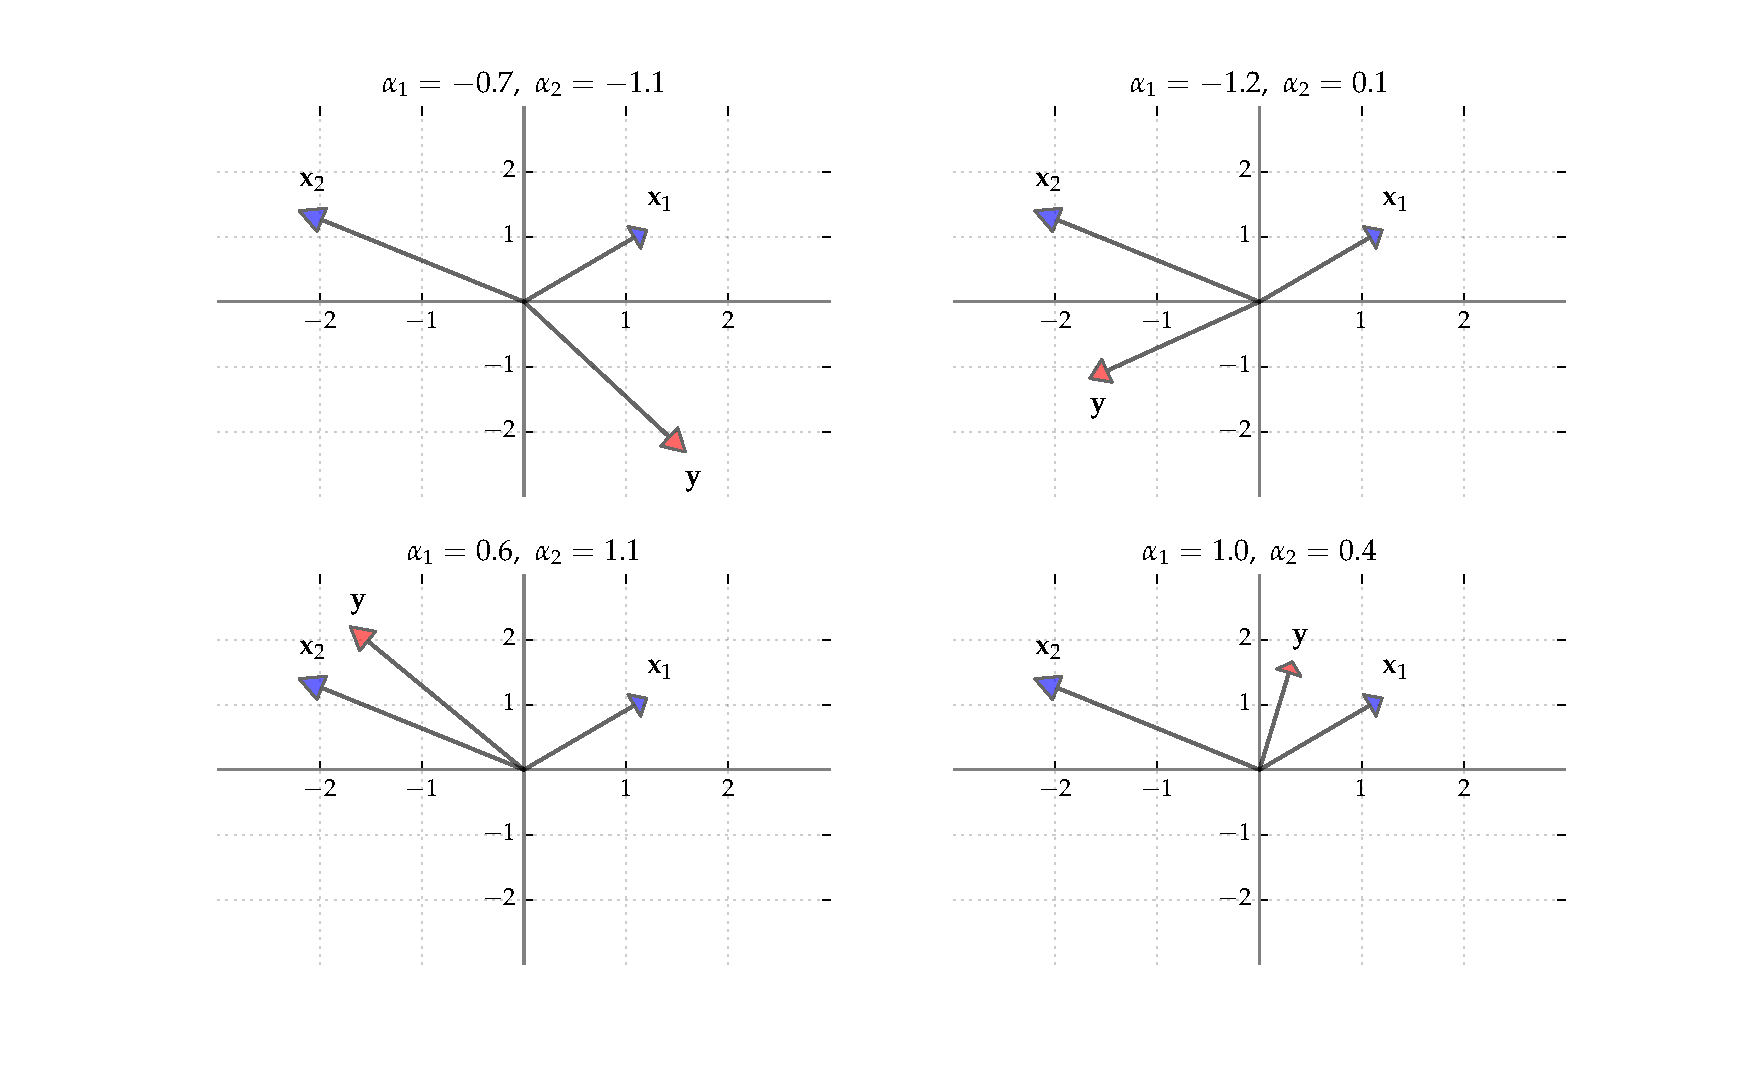
\includegraphics[trim={4em 4em 4em 1em}, clip]{lin_comb.pdf}}
        \caption{\label{f:lin_comb} Linear combinations of $\boldx_1, \boldx_2$}
       \end{center}
    \end{figure}

\end{frame}

\begin{frame}

    \frametitle{Span}

    \vspace{2em}
    Let $X \subset \RR^N$ be any nonempty set

    \vspace{1em}

    Set of all possible linear combinations of elements of $X$ is 
    called the \navy{span} of $X$, denoted by $\Span(X)$

    \vspace{.7em}

    For finite $X := \{\boldx_1,\ldots, \boldx_K\}$ the span can be expressed
    as 
    
    \begin{equation*}
        \Span(X):= \left\{ \text{ all } \sum_{k=1}^K \alpha_k \boldx_k 
        \text{ such that }
         (\alpha_1,\ldots, \alpha_K) \in \RR^K \right\}
    \end{equation*}
    
\end{frame}

\begin{frame}

    \vspace{2em}
    \Eg
    The four vectors labeled $\boldy$ 
    in the previous figure  lie
    in the span of $X = \{\boldx_1, \boldx_2\}$
    
    \vspace{.7em}
    Can \emph{any} vector in $\RR^2$ be created as a
    linear combination of $\boldx_1, \boldx_2$?  
    
    The answer is affirmative. 
    We'll prove this in \S\ref{ET-ss:bad}
    
\end{frame}



\begin{frame}
    
    \vspace{2em}
    \Eg
    Let $X = \{ \boldone \} \subset \RR^2$, where $\boldone := (1,1)$  
    
    The span of $X$ is all vectors of the form 
    %
    \[
    \alpha \boldone 
    =
    \left(
    \begin{array}{c}
        \alpha \\
        \alpha
    \end{array}
    \right)
    \quad \text{ with } \quad \alpha \in \RR  
    \]
   
    \vspace{2em}
    Constitutes a line in the plane that passes through
    %
    \begin{itemize}
        \item the vector $\boldone$  (set $\alpha = 1$)
        \item the origin $\boldzero$ (set $\alpha = 0$)
    \end{itemize}

\end{frame}

\begin{frame}

    \vspace{2em}
    \begin{figure}
       \centering
        \scalebox{.4}{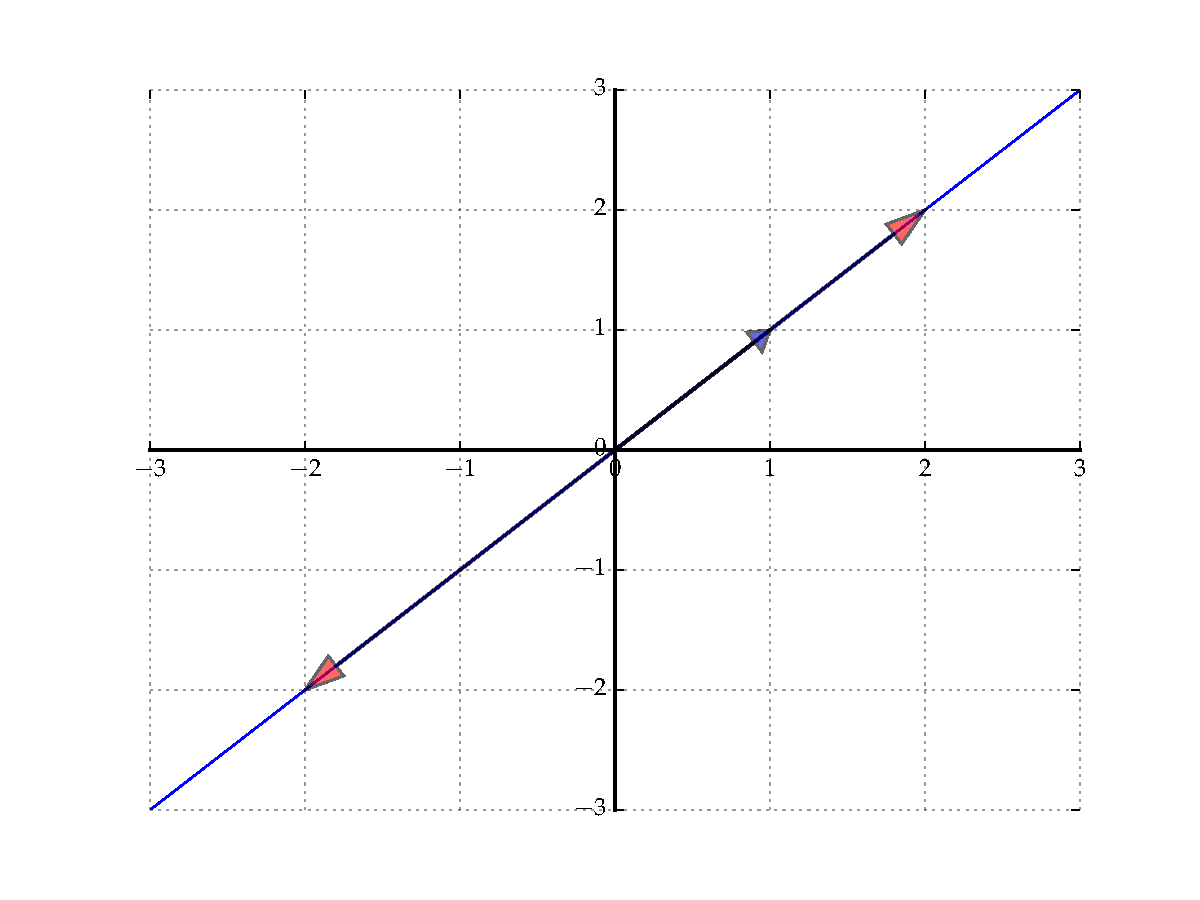
\includegraphics{span_of_one_vec.pdf}}
        \caption{The span of $\boldone := (1,1)$ in $\RR^2$}
    \end{figure}

\end{frame}

\begin{frame}
    
    \vspace{2em}
    \Eg
    The set of canonical basis vectors $\{\bolde_1, \ldots, \bolde_N\}$
    is linearly independent in $\RR^N$
    
    \Prf Let $\alpha_1, \ldots, \alpha_N$ be coefficients such that
    $\sum_{k=1}^N \alpha_k \bolde_k = \boldzero$

    Equivalently,
    %
    \begin{equation*}
        \left(
        \begin{array}{c}
            \alpha_1 \\
            \alpha_2 \\
            \vdots \\
            \alpha_N
        \end{array}
        \right)
        = \sum_{k=1}^N \alpha_k \bolde_k 
        = \boldzero
        =
        \left(
        \begin{array}{c}
            0 \\
            0 \\
            \vdots \\
            0
        \end{array}
        \right)
    \end{equation*}

    \vspace{1em}

    In particular, $\alpha_k = 0$ for all $k$
    
\end{frame}




\begin{frame}

    \vspace{2em}
    \Eg
    Let $\boldx_1 = (3, 4, 2)$ and let $\boldx_2 = (3, -4, 0.4)$

    \vspace{1em}
    By definition, the span is all vectors of the form


    \begin{equation*}
        \boldy = 
        \alpha \left(
        \begin{array}{c}
            3 \\
            4 \\
            2
        \end{array}
        \right)
        +
        \beta \left(
        \begin{array}{c}
             3 \\
             -4 \\
             0.4
        \end{array}
        \right)
        \quad \text{where} \quad
        \alpha, \beta \in \RR
    \end{equation*}
    %
    
    This is a plane that passes through
    %
    \begin{itemize}
        \item the vector $\boldx_1$
        \item the vector $\boldx_2$
        \item the origin $\boldzero$
    \end{itemize}


\end{frame}


\begin{frame}

    \vspace{2em}
   \begin{figure}
       \scalebox{.40}{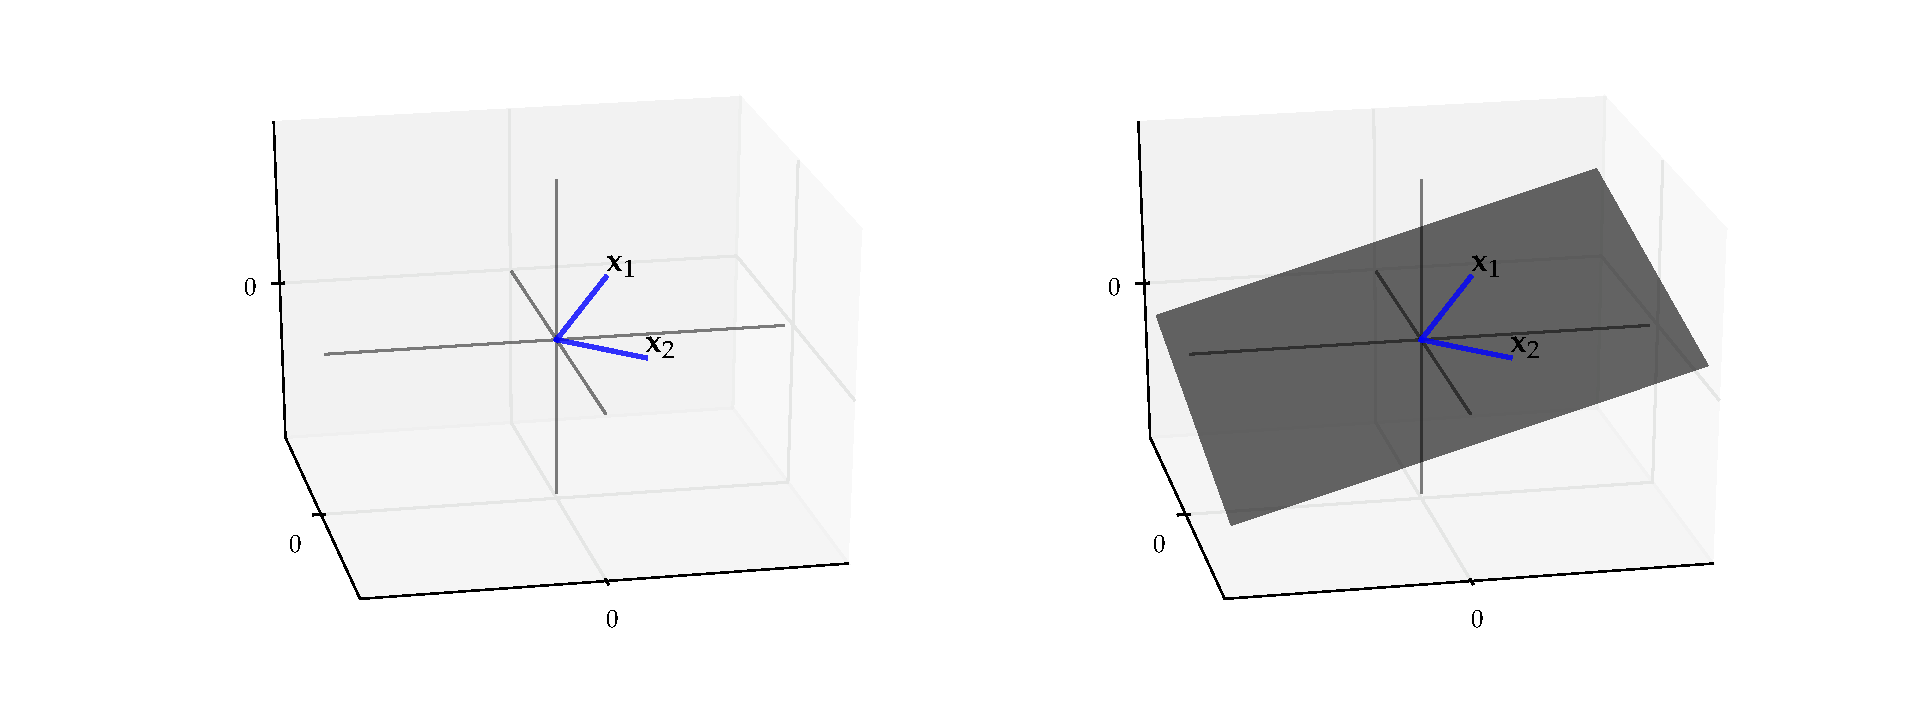
\includegraphics[trim=110 0 50 10, clip]{span_plane.pdf}}
       \caption{\label{f:span_plane} Span of $\boldx_1, \boldx_2$}
   \end{figure}

\end{frame}




%\begin{frame}
    
%    Let $Y$ be any subset of $\RR^N$, and let $X:= \{\boldx_1,\ldots, \boldx_K\}$ 
%    
%    \vspace{1em}
%
%   If $Y \subset \Span(X)$, we say that the vectors in $X$ \navy{span the set} $Y$
    
%    \vspace{1em}

 %   Alternatively, we say that $X$ is a \navy{spanning set} for $Y$

%    \vspace{1em}
    
%    A nice situation: $Y$ is large but $X$ is small
    
%    \vspace{1em}
%    $\implies$ large set $Y$ ``described'' by the small number of vectors in $X$
%\end{frame}


\begin{frame}
    
    \vspace{2em}
    \Eg 
    Consider the vectors $\{\bolde_1, \ldots, \bolde_N\} \subset \RR^N$, where

    \begin{equation*}
        \bolde_1 := 
        \left(
        \begin{array}{c}
            1 \\
            0 \\
            \vdots \\
            0
        \end{array}
        \right),
        \quad 
        \bolde_2 := 
        \left(
        \begin{array}{c}
            0 \\
            1 \\
            \vdots \\
            0
        \end{array}
        \right),
        \; 
        \cdots,
        \;
        \bolde_N := 
        \left(
        \begin{array}{c}
            0 \\
            0 \\
            \vdots \\
            1
        \end{array}
        \right)
    \end{equation*}
    %

    \vspace{1em}

    That is, $\bolde_n$ has all zeros except for a $1$ as the $n$-th element
    
    \vspace{1em}

    Vectors $\bolde_1, \ldots, \bolde_N$ are called the
    \navy{canonical basis vectors} of $\RR^N$

\end{frame}

\begin{frame}

    \begin{figure}
       \begin{center}
        \begin{tikzpicture}[
    scale=5,
    axis/.style={<->, >=stealth'},
    important line/.style={thick},
    dashed line/.style={dashed, thin},
    every node/.style={color=black}
    ]

    % define x,y
    \coordinate(O) at (0,0);
    \coordinate (X) at (0.7,0.4);
    \coordinate (e1) at (0.5,0);
    \coordinate (e2) at (0,0.5);
    % axis
    \draw[axis] (-0.3,0)  -- (0.9,0) node(xline)[right] {};
    \draw[axis] (0,-0.2) -- (0,0.7) node(yline)[above] {};
    % x, y, x+y
    \draw[important line, ->]  (O) -- (e1) node[above, text width=5em] {$\bolde_1 = (1,0)$};
    \draw[important line, ->]  (O) -- (e2) node[right, text width=5em] {$\bolde_2 = (0,1)$};
    \draw[important line, red, ->]  (O) -- (X) node[right] {$\boldy = y_1 \bolde_1 + y_2 \bolde_2$};
\end{tikzpicture}

        \caption{\label{f:vec_canon} Canonical basis vectors in $\RR^2$}
       \end{center}
    \end{figure}

\end{frame}


\begin{frame}
    
    \vspace{2em}
    \Eg (cont.) 
    
    The span of $\{\bolde_1, \ldots, \bolde_N\}$ is equal
    to all of $\RR^N$
    
    Proof for $N=2$: 
    
    Pick any $\boldy \in \RR^2$, we have
    %
    \begin{align*}
        \boldy 
        :=
        \left(
        \begin{array}{c}
            y_1 \\
            y_2
        \end{array}
        \right)
        & =
        \left(
        \begin{array}{c}
            y_1 \\
            0
        \end{array}
        \right)
        +
        \left(
        \begin{array}{c}
            0 \\
            y_1
        \end{array}
        \right)
        \\
        & =
        y_1
        \left(
        \begin{array}{c}
            1 \\
            0
        \end{array}
        \right)
        +
        y_2
        \left(
        \begin{array}{c}
            0 \\
            1
        \end{array}
        \right)
        = y_1 \bolde_1 + y_2 \bolde_2
    \end{align*}
    %
    Thus, $\boldy \in \Span \{\bolde_1, \bolde_2\}$ 
    
    Since $\boldy$ arbitrary, we have shown $\Span \{\bolde_1,
    \bolde_2\} = \RR^2$

\end{frame}

%\begin{frame}
    
    %\begin{figure}
    %   \begin{center}
     %   \scalebox{.95}{\begin{tikzpicture}[
    scale=5,
    axis/.style={<->, >=stealth'},
    important line/.style={thick},
    dashed line/.style={dashed, thin},
    every node/.style={color=black}
    ]

    % define x,y
    \coordinate(O) at (0,0);
    \coordinate (X) at (0.7,0.4);
    \coordinate (e1) at (0.5,0);
    \coordinate (e2) at (0,0.5);
    % axis
    \draw[axis] (-0.3,0)  -- (0.9,0) node(xline)[right] {};
    \draw[axis] (0,-0.2) -- (0,0.7) node(yline)[above] {};
    % x, y, x+y
    \draw[important line, ->]  (O) -- (e1) node[above, text width=5em] {$\bolde_1 = (1,0)$};
    \draw[important line, ->]  (O) -- (e2) node[right, text width=5em] {$\bolde_2 = (0,1)$};
    \draw[important line, red, ->]  (O) -- (X) node[right] {$\boldy = y_1 \bolde_1 + y_2 \bolde_2$};
\end{tikzpicture}
}
     %   \caption{\label{f:vec_canon2} Canonical basis vectors in $\RR^2$}
    %   \end{center}
   % \end{figure}

%\end{frame}


\begin{frame}
    
    \vspace{2em}
    \Eg 
    Consider the set 
    %
    \begin{equation*}
        P := \setntn{(x_1, x_2, 0) \in \RR^3}{ x_1, x_2 \in \RR}
    \end{equation*}
    %
    Graphically, $P =$ flat plane in $\RR^3$, where height
    coordinate $=0$
    %
    \begin{figure}
       \begin{center}
        \scalebox{.35}{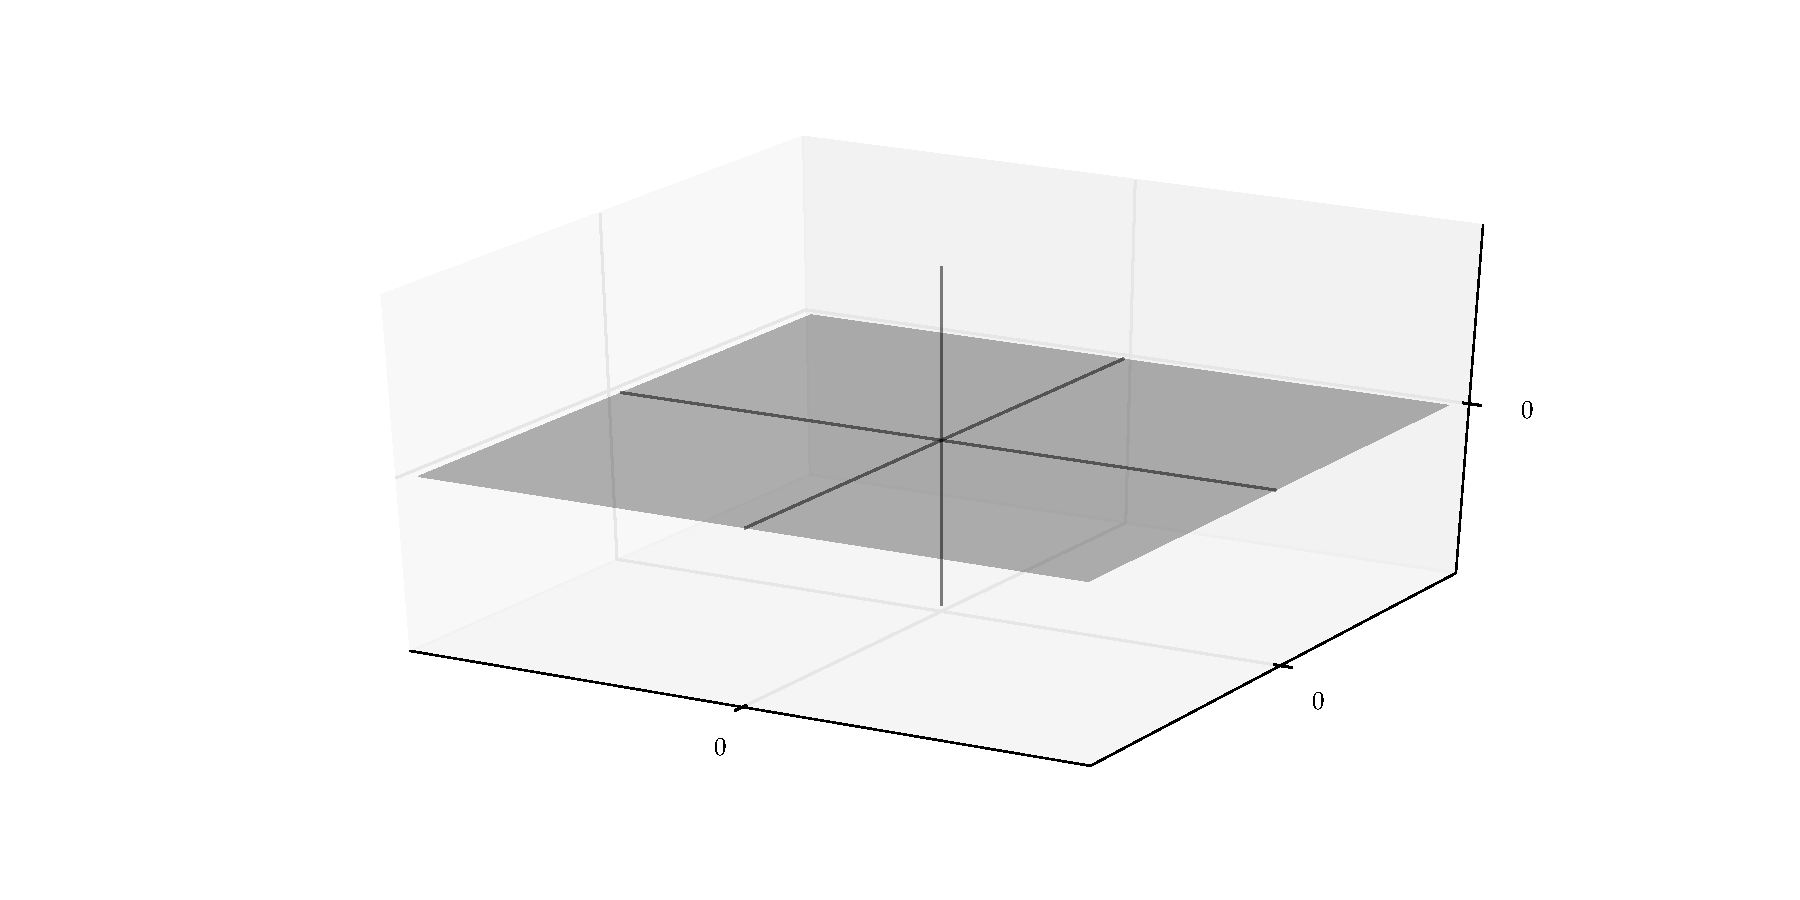
\includegraphics[trim={4em 6em 4em 1em}, clip]{flat_plane_no_vecs.pdf}}
       \end{center}
    \end{figure}

\end{frame}



\begin{frame}

    \vspace{2em}
    \Eg (cont.)
    
    If $\bolde_1 = (1,0,0)$ and $\bolde_2=(0,1,0)$, then $\Span\{\bolde_1, \bolde_2\} = P$ 
    
   To verify the claim, let $\boldx = (x_1, x_2, 0)$ be any element of $P$. 
   We can write $\boldx$ as  
    %
    \begin{equation*}
        \boldx = 
        \left(
        \begin{array}{c}
            x_1 \\
            x_2 \\
            0
        \end{array}
        \right)
        =
        x_1
        \left(
        \begin{array}{c}
            1 \\
            0 \\
            0
        \end{array}
        \right)
        + 
        x_2
        \left(
        \begin{array}{c}
            0 \\
            1 \\
            0
        \end{array}
        \right)
        = x_1 \bolde_1 + x_2 \bolde_2
    \end{equation*}
    %

    In other words, $P \subset \Span\{\bolde_1, \bolde_2\}$

    Conversely we have $\Span\{\bolde_1, \bolde_2\} \subset P$ (why?)


\end{frame}


\begin{frame}

    \vspace{2em}
    \begin{figure}
       \begin{center}
        \scalebox{.4}{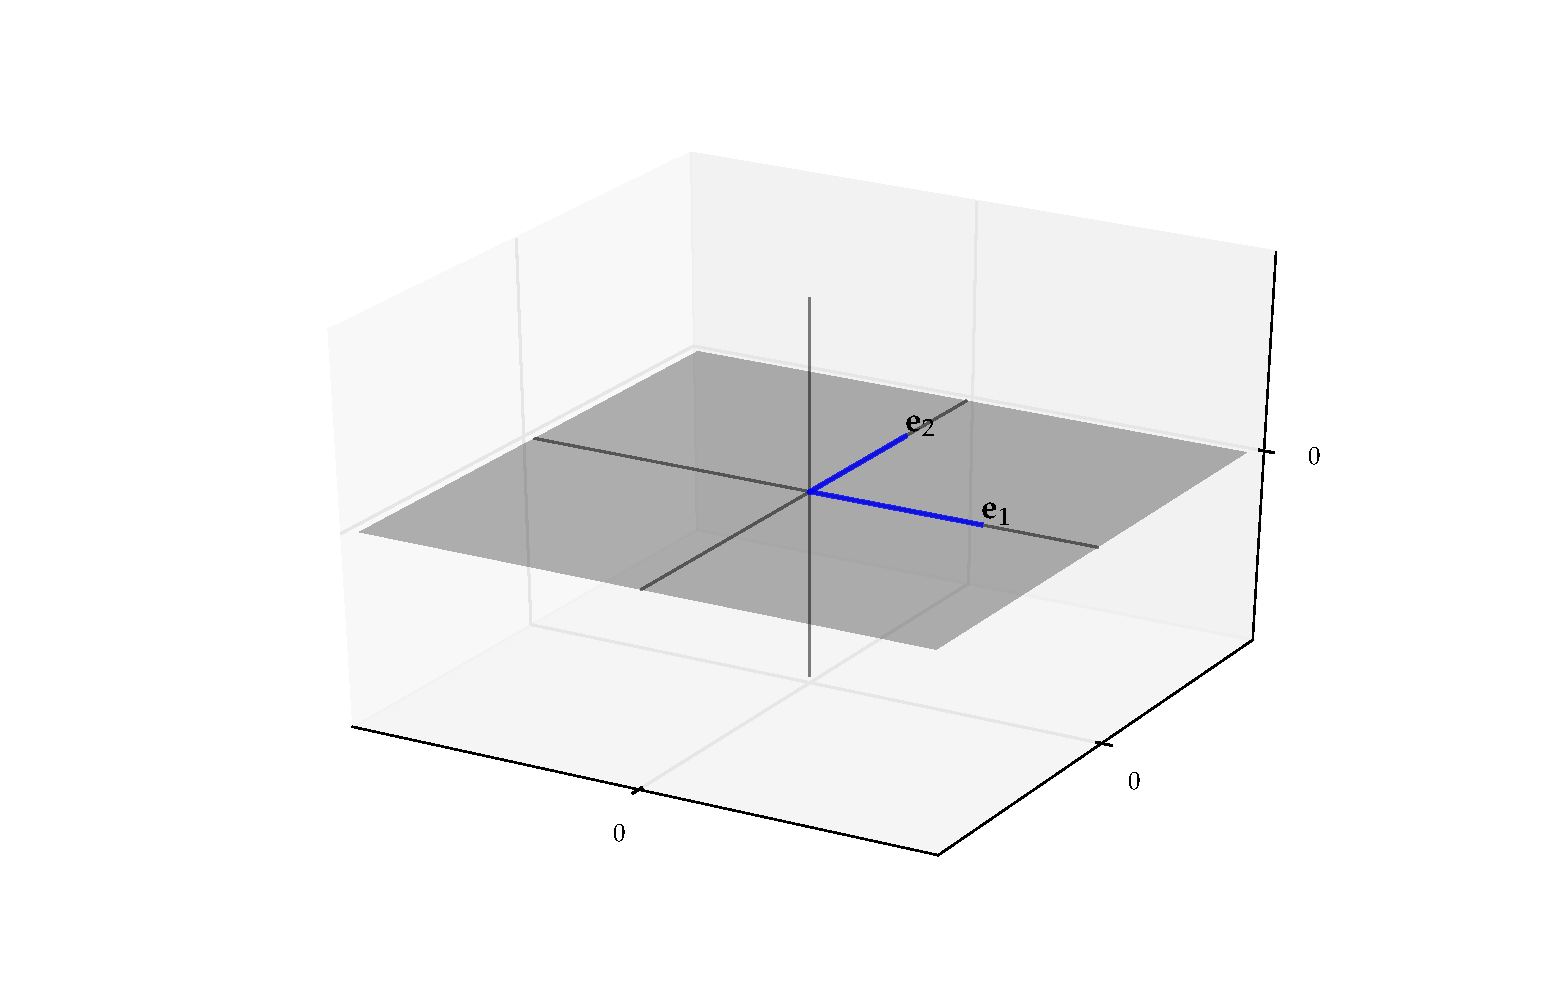
\includegraphics[trim={4em 4em 4em 1em}, clip]{flat_plane_e_vecs.pdf}}
       \end{center}
       \caption{$\Span\{\bolde_1, \bolde_2\} = P$}
    \end{figure}


\end{frame}

\begin{frame}
    
    \vspace{2em}
    \Fact{\eqref{ET-fa:xsys}} 
    If $X$ and $Y$ are non-empty subsets of $\mathbb{R}^{N}$ and $X \subset Y$, 
    then $\Span(X) \subset \Span(Y)$
    \vspace{2em}
    
    \Prf
    Pick any nonempty $X \subset Y \subset \RR^N$
    
    Let $\boldz \in \Span(X)$, we have
    %
    \begin{equation*}
        \boldz = \sum_{k=1}^K \alpha_k \boldx_k 
        \text{ for some }
        \boldx_1, \ldots, \boldx_K \in X, \; 
        \alpha_1, \ldots, \alpha_K \in \RR
    \end{equation*}
    
\end{frame}

\begin{frame}

   \vspace{2em}
    \Prf(cont.)
    Since $X \subset Y$, each $\boldx_k$ is also in $Y$, giving us
    %
    \begin{equation*}
        \boldz = \sum_{k=1}^K \alpha_k \boldx_k 
        \text{ for some }
        \boldx_1, \ldots, \boldx_K \in Y, \; 
        \alpha_1, \ldots, \alpha_K \in \RR
    \end{equation*}

    \vspace{.7em}
    Hence $\boldz \in \Span(Y)$

\end{frame}


\begin{frame}
    \frametitle{Linear Independence}
    
    \vspace{2em}
    Important applied questions:

    \begin{itemize}
        \item When is a matrix invertible?
        \item When do regression arguments suffer from collinearity?
        \item When does a set of linear equations have a solution?
    \end{itemize}

    All of these questions closely related to linear independence 

\end{frame}


\begin{frame}

    \vspace{2em}
    \frametitle{Definition}

    A nonempty collection of vectors $X := \{\boldx_1,\ldots, \boldx_K\}
    \subset \RR^N$ is called \navy{linearly independent} if
    %
    \begin{equation*}
        \sum_{k=1}^K \alpha_k \boldx_k
         = \boldzero 
        \; \implies \;
        \alpha_1 = \cdots = \alpha_K = 0
    \end{equation*}

    \vspace{1em}
    
    Informally, linearly independent sets span large spaces

\end{frame}


\begin{frame}
    
    \vspace{2em}
    \Eg 
    Consider the two vectors $\boldx_1 = (1.2, 1.1)$ and $\boldx_2 = (-2.2, 1.4)$
    
    Suppose $\alpha_1$ and $\alpha_2$ are scalars with
    %
    \begin{equation*}
        \alpha_1
        \left(
        \begin{array}{c}
            1.2 \\
            1.1
        \end{array}
        \right)
        + 
        \alpha_2
        \left(
        \begin{array}{c}
            -2.2 \\
            1.4
        \end{array}
        \right)
        =
        \boldzero
    \end{equation*}
    
    This translates to a linear, two-equation system, where the unknowns
    are $\alpha_1$ and $\alpha_2$ 
    
    The only solution is $\alpha_1 = \alpha_2 = 0$
    
    $\{\boldx_1, \boldx_2\}$ is linearly independent


\end{frame}

    \begin{frame}
        \begin{figure}
       \begin{center}
           \scalebox{.46}{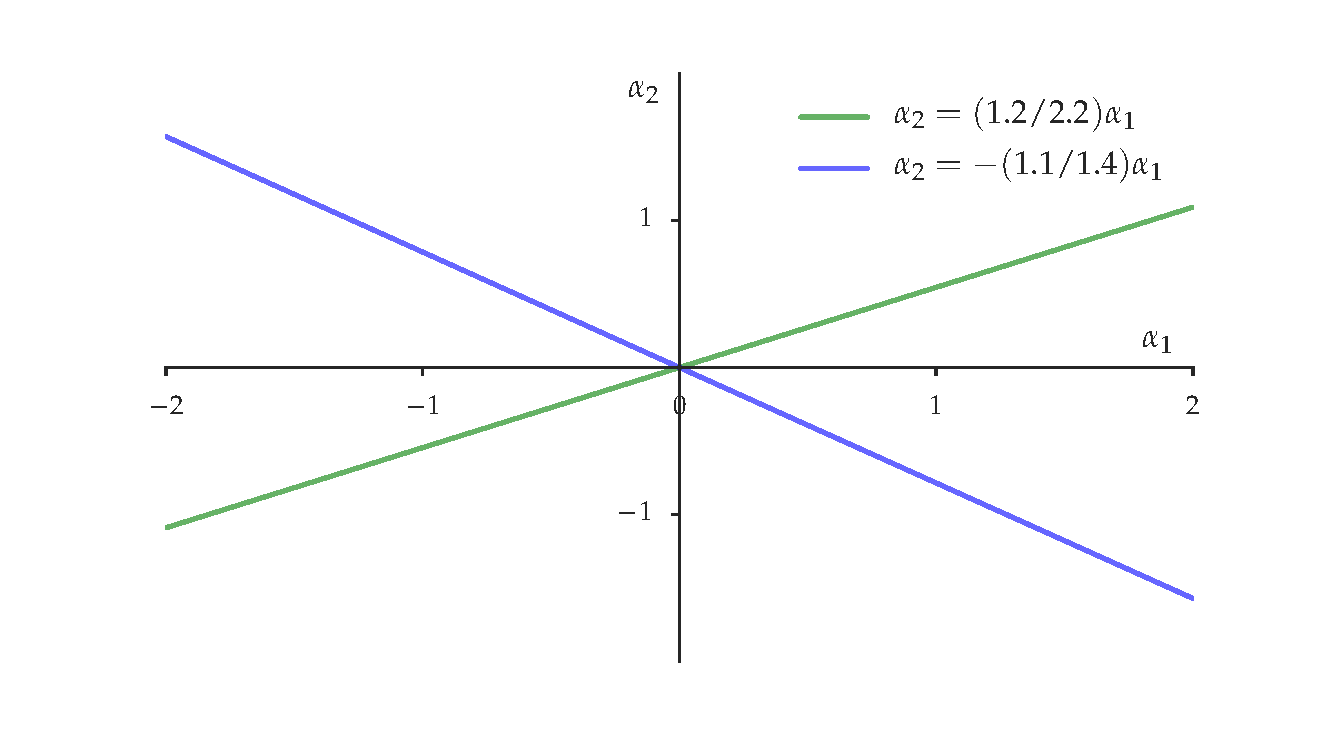
\includegraphics[trim={0 4em 0 1em}, clip]{alpha_eq.pdf}}
           \caption{\label{f:alpha_eq} The only solution is $\alpha_1 = \alpha_2 = 0$}
       \end{center}
    \end{figure}

\end{frame}

\begin{frame}
    
    \vspace{2em}
    \Eg The set of canonical basis vectors $\{\bolde_1, \ldots, \bolde_N\}$
    is linearly independent in $\RR^N$

    To see this, let $\alpha_1, \ldots, \alpha_N$ be coefficients such that
    $\sum_{k=1}^N \alpha_k \bolde_k = \boldzero$. We have
    %
    \begin{equation*}
        \left(
        \begin{array}{c}
            \alpha_1 \\
            \alpha_2 \\
            \vdots \\
            \alpha_N
        \end{array}
        \right)
        = \sum_{k=1}^N \alpha_k \bolde_k 
        = \boldzero
        =
        \left(
        \begin{array}{c}
            0 \\
            0 \\
            \vdots \\
            0
        \end{array}
        \right)
    \end{equation*}

    In particular, $\alpha_k = 0$ for all $k$
    
    Hence  $\{\bolde_1, \ldots, \bolde_N\}$ linearly independent

\end{frame}

\begin{frame}

    \vspace{2em}
    \Thm\eqref{ET-t:fdlinin}
        Let $X := \{\boldx_1,\ldots, \boldx_K\} \subset \RR^N$.  For $K > 1$, the
        following statements are equivalent:
        %
        \begin{enumerate}
            \item $X$ is linearly independent
            \item $X_0$ is a proper subset of $X$
                $\,\implies\,$ $\Span X_0$ is a proper subset of $\Span X$
            \item No vector in $X$ can be written as a linear combination of the others
        \end{enumerate}
        %
    Proof is an exercise. See ET ex. \ref{ET-ex:ott} and solution
    
\end{frame}

\begin{frame}

    \vspace{2em}
    \Eg 
    Dropping any of the canonical basis vectors reduces span

    Consider the $N=2$ case
    
    We know $\Span \{\bolde_1, \bolde_2\} = \RR^2$
    
    \begin{itemize}
    \item removing either element of $\Span \{\bolde_1, \bolde_2\}$ reduces the span to a line
    \end{itemize}
    
\end{frame}

\begin{frame}

    \vspace{2em}
    However, let $\boldx_1 = (1,0)$ and $\boldx_2 = (-2,0)$
    
    \vspace{1em}
    The pair are not linearly independent since $\boldx_2 = -2\boldx_1$
        \begin{itemize}
            \item dropping
                either vector does not change the span---the span remains the horizontal axis 
            \item we have $\boldx_2 = -2
            \boldx_1$, which means that each vector can be written as a linear combination
            of the other
        \end{itemize}
        
        \begin{center}
            \begin{tikzpicture}[
    scale=5,
    axis/.style={<->, >=stealth'},
    important line/.style={thick,color=blue},
    dashed line/.style={dashed, thin},
    every node/.style={color=black}
    ]

    % define x,y
    \coordinate(O) at (0,0);
    \coordinate (e1) at (0.2,0);
    \coordinate (x) at (-0.4,0);
    % axis
    \draw[axis] (-1,0)  -- (1,0) node(xline)[right] {};
    \draw[axis] (0,-0.2) -- (0,0.2) node(yline)[above] {};
    % x, y, x+y
    \draw[important line, ->]  (O) -- (e1) node[anchor = south west, text width=5em] {$\boldx_1 = (1,0)$};
    \draw[important line, ->]  (O) -- (x) node[below, text width=6em] {$\boldx_2 = (-2,0)$};
\end{tikzpicture}

        \end{center}
 \end{frame}


\begin{frame}

    \vspace{2em}
    \Fact\eqref{ET-fa:slili}
        If $X := \{\boldx_1,\ldots, \boldx_K\}$ is linearly independent, then
        %
        \begin{enumerate}
            \item every subset of $X$ is linearly independent, 
            \item $X$ does not contain $\boldzero$, and
            \item $X \cup \{ \boldx \}$ is linearly independent for all $\boldx
                \in \RR^N$ such that $\boldx \notin \Span X$.
        \end{enumerate}
        %
   
    The proof is a solved exercise (ex.~\ref{ET-ex:slili} in ET)
\end{frame}

\begin{frame}\frametitle{Linear Independence and Uniqueness}
    
    \vspace{2em}
    Linear independence is the key condition for existence \emph{and} 
    uniqueness of solutions to system of linear equations 
    
    \vspace{.7em}
    \Thm\eqref{ET-t:unor}
    Let $X := \{\boldx_1,\ldots,\boldx_K\}$ be any collection of vectors in
    $\RR^N$.  The following statements are equivalent:
    %
    \begin{enumerate}
        \item $X$ is linearly independent  
        \item For each $\boldy \in \RR^N$
            there exists at most one set of scalars $\alpha_1,\ldots,\alpha_K$
            such that 
            %
            \begin{equation}
                \label{eq:yilcx}
                \boldy =  
                \alpha_1 \boldx_1
                + \cdots +
                \alpha_K \boldx_K
            \end{equation}
            %
    \end{enumerate}
    %    
\end{frame}

\begin{frame}

    \vspace{2em}
    \Prf 
    (1. $\implies$ 2.)
    
    Let $X$ be linearly independent and pick any $\boldy$  
    
    Suppose by contradiction that \eqref{eq:yilcx} holds for more than one set of scalars; we have
    %
    \begin{equation*}
        \exists \;
        \alpha_1, \ldots, \alpha_K
        \text{ and } \beta_1, \ldots, \beta_K
        \; \st \; 
        \boldy 
        = \sum_{k=1}^K \alpha_k \boldx_k
        = \sum_{k=1}^K \beta_k \boldx_k
    \end{equation*}
    %
    \begin{equation*}
        \fore \sum_{k=1}^K (\alpha_k - \beta_k) \boldx_k = \boldzero
    \end{equation*} 
    %
    \begin{equation*}
        \fore
        \alpha_k = \beta_k 
        \quad \text{for all} \quad k
    \end{equation*}
 
\end{frame}

\begin{frame}
    
    \Prf (2. $\implies$1.)
    
    If 2. holds, then there exists at most one set of scalars such that \[\boldzero =
    \sum_{k=1}^K \alpha_k \boldx_k\]
    
    Because $\alpha_1 = \cdots = \alpha_k = 0$
    has this property, no nonzero scalars yield $\boldzero =
    \sum_{k=1}^K \alpha_k \boldx_k$
    
    We can then conclude $X$ is linearly
    independent, by the definition of linear independence 
    

\end{frame}


\begin{frame}\frametitle{Linear Subspaces}

    \vspace{2em}
    A  nonempty subset $S$ of $\RR^N$ is called a \navy{linear subspace} (or just
    \navy{subspace}) of $\RR^N$
    if
    %
    \begin{equation*}
        \label{eq:lsubd}
        \boldx, \, \boldy \in S
        \text{ and } \alpha, \, \beta \in \RR
        \; \implies \; 
        \alpha \boldx + \beta \boldy \in S
    \end{equation*}
    %
    In other words, $S\subset \mathbb{R}^{N}$ is ``closed" under vector addition
     and scalar multiplication 
    
    \vspace{2em}
    \Eg 
    If $X$ is any
    nonempty subset of $\RR^N$, then $\Span X$ is a linear subspace of
    $\RR^N$

\end{frame}

\begin{frame}

    \vspace{2em}
    \Eg 
    $\mathbb{R}^{N}$ is a linear subspace of $\mathbb{R}^{N}$
    
    \vspace{.7em}
    \Eg 
    Given any $\bolda \in \RR^N$, the set $A := \setntn{\boldx \in
    \RR^N}{\inner{\bolda, \boldx}  = 0}$
    is a linear subspace of $\RR^N$
    
    \vspace{2em}
    To see this, let $\boldx, \boldy \in A$, let $\alpha, \beta \in \RR$ and 
    define $\boldz := \alpha \boldx + \beta \boldy \in A$
    
    We have 
        %
        $$
        \inner{\bolda, \boldz} =
        \inner{\bolda, \alpha \boldx + \beta \boldy} 
        = \alpha \inner{ \bolda, \boldx}
        + \beta \inner{\bolda, \boldy} = 0 + 0 = 0
        $$
    Hence $\boldz\in A$


\end{frame}

\begin{frame}

    \vspace{.7em}
    \Fact\eqref{ET-fa:eplsub}
    If $S$ is a linear subspace of $\RR^N$, then
    %
    \begin{enumerate}
        \item $\boldzero \in S$
        \item $X \subset S \implies \Span X \subset S$, and
        \item $\Span S = S$
    \end{enumerate}
    \vspace{2em}
    
    \Thm\eqref{ET-t:exth}
    Let $S$ be a linear subspace of $\RR^N$. If $S$ is spanned by $K$ vectors,
    then any linearly independent subset of $S$ has at most $K$
    vectors
    
\end{frame}

\begin{frame}

    \vspace{2em}
    \Eg
    Recall the canonical basis vectors
    $\{\bolde_1, \bolde_2\}$ spanned $\RR^2$. As such, from Theorem~\ref{ET-t:exth}, 
    the three vectors below are linearly dependent 
    %
    \begin{figure}
       \begin{center}
        \scalebox{.33}{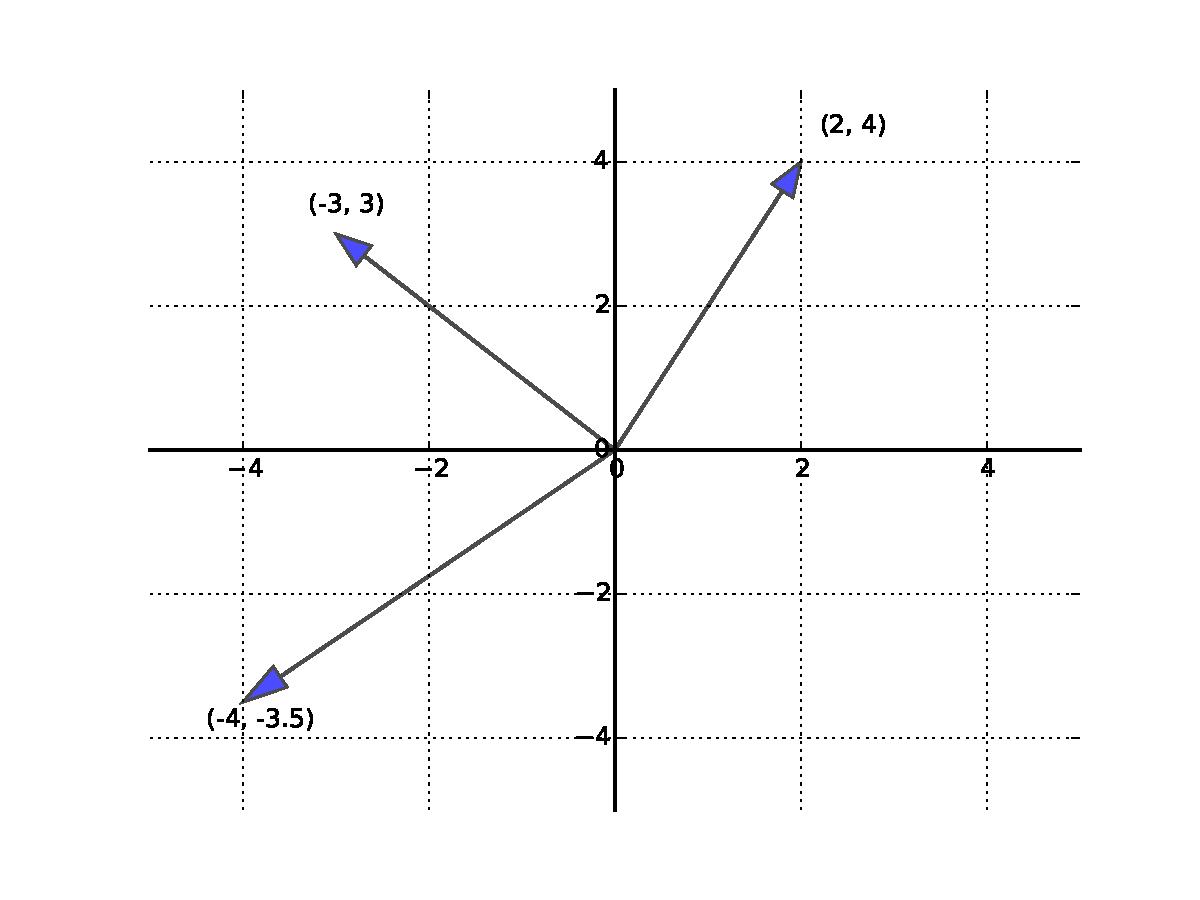
\includegraphics{vecs.pdf}}
       \end{center}
    \end{figure}
    
\end{frame}

\begin{frame}

    \vspace{2em}
    \Eg
    The plane
        $P := \setntn{(x_1, x_2, 0) \in \RR^3}{ x_1, x_2 \in \RR}$
    from example~\ref{ET-eg:planein3d} in ET can be
    spanned by two vectors
    
    By theorem~\ref{ET-t:exth}, the three vectors in the
    figure below are linearly dependent 
    %
    \begin{figure}
       \begin{center}
           \scalebox{.4}{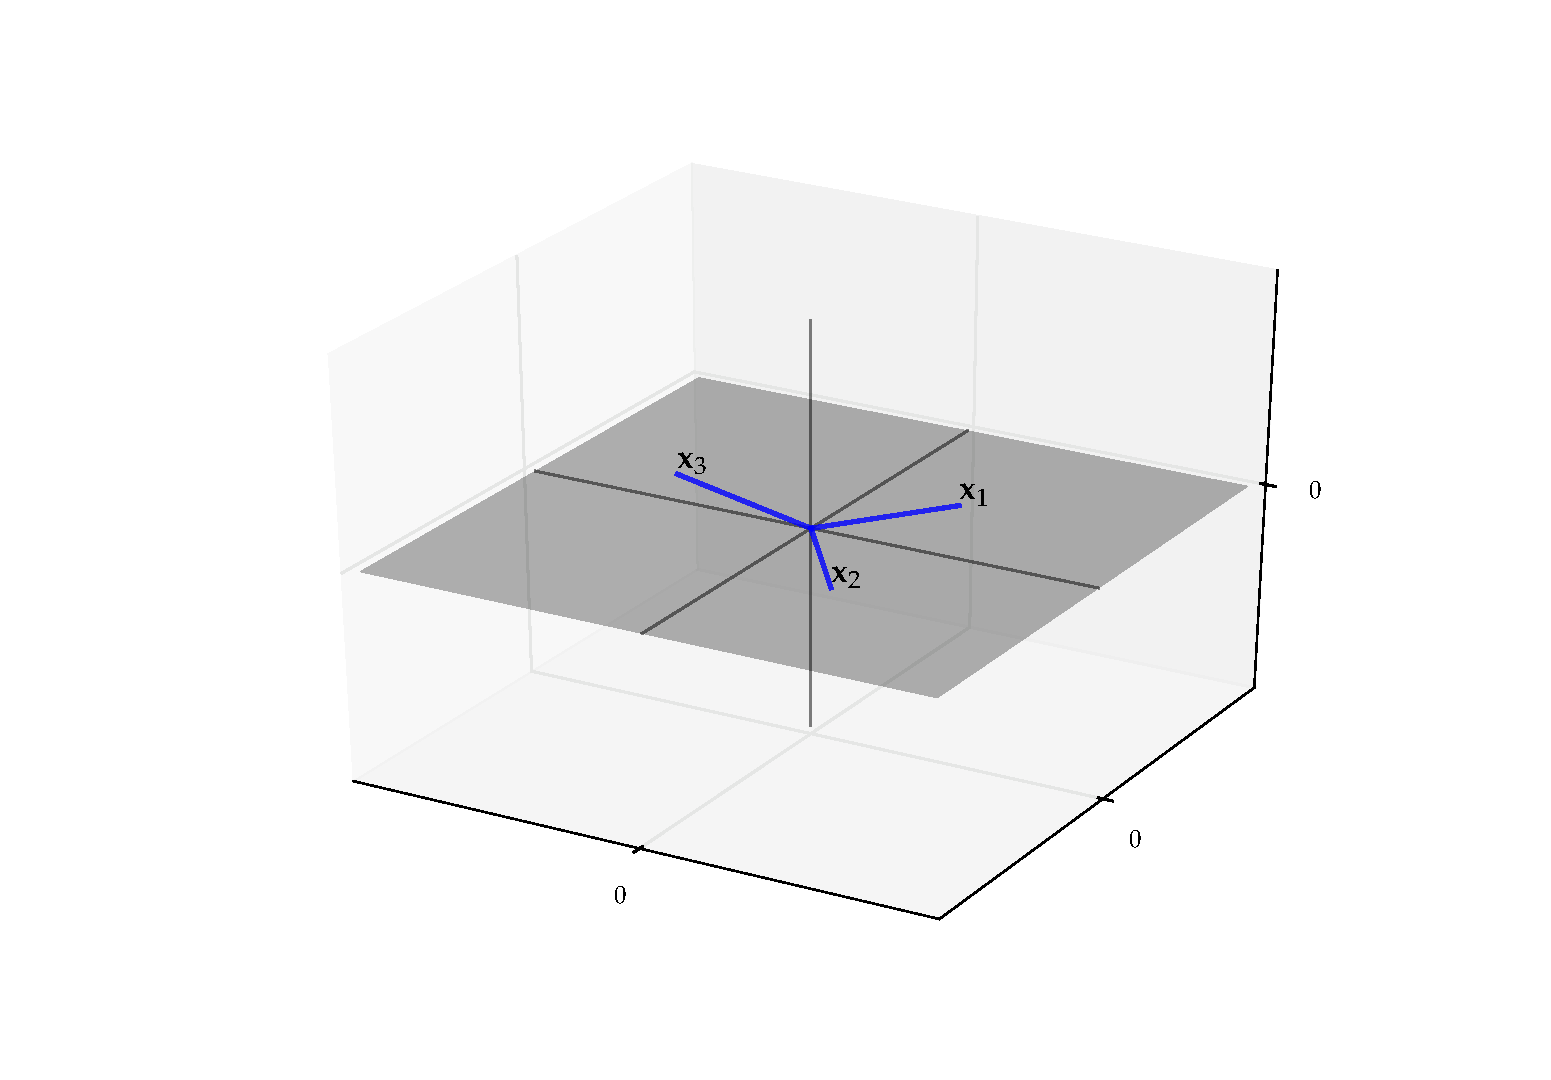
\includegraphics[trim={0 5em 0 15em}, clip]{flat_plane.pdf}}
       \end{center}
    \end{figure}

\end{frame}

\begin{frame}\frametitle{Bases and Dimension}

    \vspace{2em}
    \Thm\eqref{ET-t:bsili}
        Let $X := \{ \boldx_1, \ldots, \boldx_N \}$ be any $N$ vectors in $\RR^N$.
        The following statements are equivalent:
        %
        \begin{enumerate}
            \item $\Span X = \RR^N$
            \item $X$ is linearly independent
        \end{enumerate}
    
    \vspace{.7em}
    For a proof see page~\pageref{ET-t:bsili} in ET
    
\end{frame}

\begin{frame}

    \vspace{2em}
    Let $S$ be a linear subspace of $\RR^N$ and
    let $B \subset S$
    
    \vspace{.7em}
    The set $B$ is called a \navy{basis} of $S$
    if 
    %
    \begin{enumerate}
        \item $B$ spans $S$ and
        \item $B$ is linearly independent
    \end{enumerate}
    
    \vspace{.7em}
    The plural of basis is \navy{bases}
    
\end{frame}

\begin{frame}
    
    \vspace{2em}
    From theorem~\ref{ET-t:unor}, when
    $B$ is a basis of $S$, each point in $S$ has exactly one representation as a
    linear combination of elements of $B$
    
    \vspace{.7em}
    From theorem~\ref{ET-t:bsili}, any $N$ linearly
    independent vectors in $\RR^N$ form a basis of $\RR^N$
    
\end{frame}

\begin{frame}
    
    \vspace{2em}
    \Eg
    Recall the plane from the example above
    %
    \begin{equation*}
        P := \setntn{(x_1, x_2, 0) \in \RR^3}{ x_1, x_2 \in \RR}
    \end{equation*}
    %
    We showed $\Span\{\bolde_1, \bolde_2\} = P$ for 
    %
    \begin{equation*}
        \bolde_1 := 
        \left(
        \begin{array}{c}
            1 \\
            0 \\
            0
        \end{array}
        \right),
        \quad 
        \bolde_2 := 
        \left(
        \begin{array}{c}
            0 \\
            1 \\
            0
        \end{array}
        \right)
    \end{equation*}
    %
    
    Moreover, $\{\bolde_1, \bolde_2\}$ is linearly independent (why?)

    Hence $\{\bolde_1, \bolde_2\}$ is a basis for $P$


\end{frame}

\begin{frame}

    \vspace{2em}
    \Thm{\eqref{ET-t:basis}}
    If $S$ is a linear subspace of $\RR^N$ distinct from $\{\boldzero\}$, then 
    %
    \begin{enumerate}
        \item $S$ has at least one basis and
        \item every basis of $S$ has the same number of elements.
    \end{enumerate}
    %
    If $S$ is a linear subspace of $\RR^N$, then the common number identified in
    theorem~\ref{ET-t:basis} is called the \navy{dimension} of $S$, and written as
    $\dim S$
    
\end{frame}

\begin{frame}
    
    \vspace{2em}
    \Eg
    For $P := \setntn{(x_1, x_2, 0) \in \RR^3}{ x_1, x_2 \in \RR}$, $\dim P = 2$ because 
    %
    \begin{equation*}
        \bolde_1 := 
        \left(
        \begin{array}{c}
            1 \\
            0 \\
            0
        \end{array}
        \right),
        \quad 
        \bolde_2 := 
        \left(
        \begin{array}{c}
            0 \\
            1 \\
            0
        \end{array}
        \right)
    \end{equation*}
    %
    is a basis with two elements
    
    \vspace{.7em}
    \Eg
    A line $\setntn{\alpha \boldx \in \RR^N}{\alpha \in \RR}$ through
    the origin is one dimensional
    
\end{frame}

\begin{frame}

    \vspace{2em}
    In $\RR^N$ the singleton subspace $\{\boldzero\}$ is said to have zero
    dimension

    If we take a set of $K$ vectors, then how large will its span be in terms
    of dimension?  
    
    \vspace{.7em}
    \Thm\eqref{ET-t:dimspan}
        If $X := \{\boldx_1,\ldots,\boldx_K\} \subset \RR^N$, then
        %
        \begin{enumerate}
            \item $\dim \Span X \leq K$ and
            \item $\dim \Span X = K$ if and only if $X$ is linearly independent.
        \end{enumerate}
        %
    For a proof, see exercise~\ref{ET-ex:dimspan} in ET
    
\end{frame}

\begin{frame}

    \vspace{2em}
    \Fact{\eqref{ET-fa:ondsrn}}
        The following statements are true:
        %
        \begin{enumerate}
            \item Let $S$ and $S'$ be $K$-dimensional linear subspaces of $\RR^N$. If $S
                \subset S'$, then $S = S'$
            \item If $S$ is an $M$-dimensional linear subspace of $\RR^N$ and $M
                < N$, then $S \not= \RR^N$
        \end{enumerate}
        %
        
\end{frame}



\begin{frame}\frametitle{Linear Maps}

    \vspace{2em}
    A function $T \colon \RR^K \to \RR^N$ is called
    \navy{linear} if 
    %
    \begin{equation*}
            T(\alpha \boldx + \beta \boldy) = \alpha T\boldx + \beta T\boldy
            \qquad
            \forall \, 
            \boldx, \boldy \in \RR^K, \;
            \forall \,
            \alpha, \beta \in \RR
    \end{equation*}
    %

    \vspace{.7em}
    Notation: 
    
    \begin{itemize}
        \item Linear functions often written with upper case letters
            \vspace{0.5em}
        \item Typically omit parenthesis around arguments when convenient
    \end{itemize}

\end{frame}

\begin{frame}

    \vspace{2em}
   \Eg $T \colon \RR \to \RR$ defined by $Tx = 2x$ is linear 

    To see this, take any $\alpha, \beta, x, y$ in $\RR$ and observe 
    %
    \begin{equation*}
      T(\alpha x + \beta y)
      = 2(\alpha x + \beta y)
      = \alpha 2 x + \beta 2 y
      = \alpha Tx + \beta Ty  
    \end{equation*}

    \vspace{.7em}
    \Eg The function $f \colon \RR \to \RR$ defined by $f(x) = x^2$ is
    \underline{non}linear
    
    To see this, set $\alpha = \beta = x = y = 1$. We then have
    %
    $$f(\alpha x + \beta y) = f(2) = 4$$
    %
    However, $\alpha f(x) + \beta f(y) = 1 + 1 = 2$
    
\end{frame}

\begin{frame}
    
    \vspace{2em}
    Remark: Thinking of linear functions as those whose graph is a straight
    line is not correct
    
    \vspace{.7em}
    \Eg    
    Function $f \colon \RR \to \RR$ defined by $f(x) = 1 + 2x$ is
    \underline{non}linear

    Take $\alpha = \beta = x = y = 1$. We then have
    %
    $$f(\alpha x + \beta y) = f(2) = 5$$
    
    However, $\alpha f(x) + \beta f(y) = 3 + 3 = 6$
   
    \vspace{.7em}
    
    This kind of function is called an \navy{affine} function

\end{frame}

\begin{frame}

    \vspace{2em}
    By definition, if $T$ is linear, then the exchange of order in 
    %
    \[T [ \sum_{k=1}^K \alpha_k \boldx_k ]
    = \sum_{k=1}^K \alpha_k T \boldx_k\]
    %
    will be valid whenever $K=2$
    
    \vspace{.7em}
    Inductive argument extends this to arbitrary $K$
    
\end{frame}

\begin{frame}

    \vspace{2em}
    \Fact{\eqref{ET-fa:res}}
    If $T \colon \RR^K \to \RR^N$ is a linear map, then 
    %
    \begin{equation*}
        \range(T) = \Span(V) 
        \quad \text{where} \quad
        V := \{T\bolde_1, \ldots, T\bolde_K\}
    \end{equation*}


    where $\bolde_k$ is the $k$-th canonical basis vector in $\RR^K$
    \vspace{1em}

    \Prf Any $\boldx \in \RR^K$ can be expressed as $\sum_{k=1}^K \alpha_k \bolde_k$. 
    Hence $\range(T)$ is the set of all points of the form
    %
    \begin{equation*}
        T\boldx
        = T \left[ \sum_{k=1}^K \alpha_k \bolde_k \right]
        = \sum_{k=1}^K \alpha_k T \bolde_k 
    \end{equation*}
    %
    as we vary $\alpha_1, \ldots, \alpha_K$ over all combinations.
    This coincides with the definition of $\Span(V)$

\end{frame}

\begin{frame}
    
    \vspace{2em}
    The \navy{null space} or \navy{kernel} of linear map $T \colon \RR^K \to
    \RR^N$ is
    %
    \begin{equation*}
        \kernel(T) := \setntn{\boldx \in \RR^K}{T\boldx = \boldzero}
    \end{equation*}
    %

    \vspace{.7em}
    \Fact{\eqref{ET-fa:res}}
    If $T \colon \RR^K \to \RR^N$ is a linear map, then 
    %
    \begin{equation*}
        \range T = \Span V,
        \quad \text{where } 
        V := \{T\bolde_1, \ldots, T\bolde_K\}
    \end{equation*}
    %
    Proofs are straight-forward (complete as exercise)
    
\end{frame}

\begin{frame}
    
    \frametitle{Linear Independence and Bijections}

    \vspace{.7em}
    Many scientific and practical problems are ``inverse" problems

    \begin{itemize}
        \item we observe outcomes but not what caused them
        \item how can we work backwards from outcomes to causes?
    \end{itemize}
    
    Examples

    \begin{itemize}
        \item what consumer preferences generated observed market behavior?
        \item what kinds of expectations led to given shift in exchange rates?
    \end{itemize}

\end{frame}

\begin{frame}
    
    \vspace{2em}
    Loosely, we can express an inverse problem as
    
    \begin{figure}
       \begin{center}
        \scalebox{.5}{\input{inverse_prob.pdf_t}}
       \end{center}
    \end{figure}

    \begin{itemize}
        \item does this problem have a solution?
        \item is it unique?
    \end{itemize}

    Answers depend on whether $F$ is one-to-one, onto, etc.

    The best case is a bijection

    But other situations also arise

\end{frame}

\begin{frame}

    \vspace{2em}
    \Thm {\eqref{ET-t:linfunc}}
        If $T$ is a linear function from $\RR^N$ to $\RR^N$, then all of the
        following are equivalent:
        %
        \begin{enumerate}
            \item $T$ is a bijection.
            \item $T$ is onto.
            \item $T$ is one-to-one.
            \item $\kernel T = \{ \boldzero \}$.
            \item $V := \{T\bolde_1, \ldots, T\bolde_N\}$ is
                linearly independent.
            \item $V := \{T\bolde_1, \ldots, T\bolde_N\}$ forms a basis of
                $\RR^N$.
        \end{enumerate}
        % 
    See exercise \ref{ET-ex:linfunc} in ET for proof
    
    \vspace{.7em}
    If any one of these conditions is true, then $T$ is called
    \navy{nonsingular}. Otherwise $T$ is called \navy{singular}
    
\end{frame}

\begin{frame}

    \begin{figure}
       \begin{center}
        \scalebox{.4}{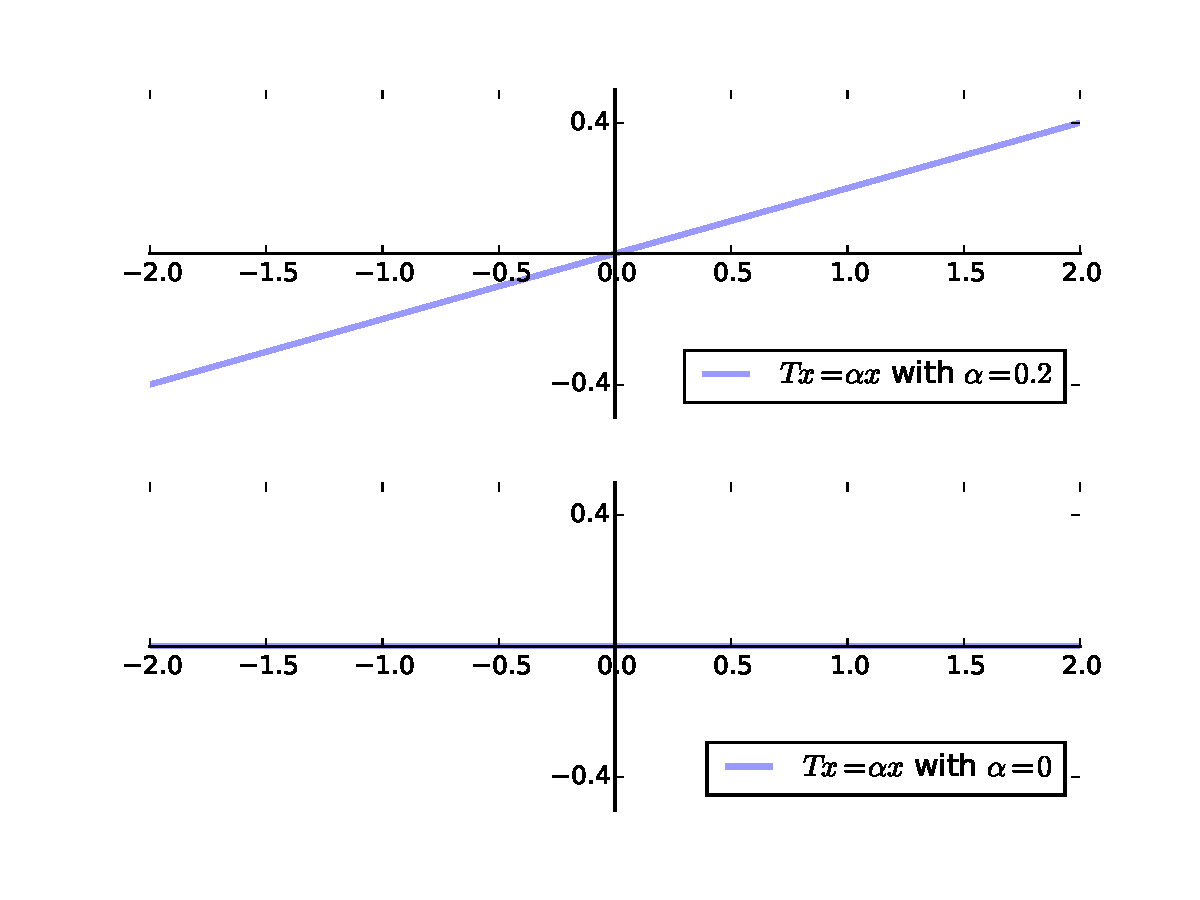
\includegraphics{linbijec.pdf}}
        \caption{The case of $N=1$, nonsingular and singular}
       \end{center}
    \end{figure}
    
\end{frame}

\begin{frame}
    
    \vspace{2em}
    If $T$ is nonsingular, then, being a bijection, it must have an inverse
    function $T^{-1}$ that is also a bijection (fact~\ref{ET-fa:bij} on
    page~\pageref{ET-fa:bij})

    \vspace{.7em}
    \Fact{\eqref{ET-fa:nsins}}
        If $T \colon \RR^N \to \RR^N$ is nonsingular, then so is $T^{-1}$.  

    For a proof, see ex.~\ref{ET-ex:nsins}
    
\end{frame}

\begin{frame}

    \frametitle{Maps Across Different Dimensions} 

    \vspace{2em}
    Remember that the above results apply to maps from $\RR^N$ to $\RR^N$

    Things change when we look at linear maps across dimensions

    \vspace{.7em}

    The general rules for linear maps are 

    \begin{itemize}
        \item maps from lower to higher dimensions cannot be onto
        \item maps from higher to lower dimensions cannot be one-to-one
    \end{itemize}

    In either case they cannot be bijections

    \vspace{1em}

\end{frame}

\begin{frame}
    
    \vspace{2em}
    \Thm{\eqref{ET-t:lfoc}}
    For a linear map $T$ from $\RR^K \to \RR^N$, the following statements are
    true:
    %
    \begin{enumerate}
        \item If $K < N$, then $T$ is not onto.
        \item If $K > N$, then $T$ is not one-to-one.
    \end{enumerate}
    %
    \Prf(part 1)
    
    Let $K < N$ and let $T \colon \RR^K \to \RR^N$ be linear  
    
    Letting $V := \{T\bolde_1, \ldots, T\bolde_K\}$, we have
    %
    $$
    \dim(\range(T)) = \dim(\Span(V)) \leq K < N
    $$
    %
    $$
    \fore 
        \range(T) \not= \RR^N
    $$
    Hence $T$ is not onto 
    
\end{frame}

\begin{frame}
    
    \Prf(part 2)
    
    Suppose to the contrary that $T$ is one-to-one

    Let $\alpha_1, \ldots, \alpha_K$ be a collection of vectors such that 
    %
    \[
    \alpha_1 T \bolde_1 + \cdots + \alpha_K T \bolde_K = \boldzero
    \]
    %
    \[
    \fore 
    T (\alpha_1 \bolde_1 + \cdots + \alpha_K \bolde_K) = \boldzero
    \qquad (\text{by linearity})
    \]
    %
    \[
    \fore
    \alpha_1 \bolde_1 + \cdots + \alpha_K \bolde_K = \boldzero
    \qquad (\text{since $\ker(T) = \{\boldzero\}$})
    \]
    %
    \[
    \fore 
    \alpha_1 = \cdots = \alpha_K = 0
    \qquad (\text{by independence of $\{\bolde_1, \ldots \bolde_K\}$)}
    \]

    We have shown that $\{T\bolde_1, \ldots, T\bolde_K\}$ is linearly
    independent

    But then $\RR^N$ contains a linearly independent set
    with $K > N$ vectors --- contradiction

\end{frame}


\begin{frame}
    
    \begin{figure}
       \begin{center}
           \scalebox{.4}{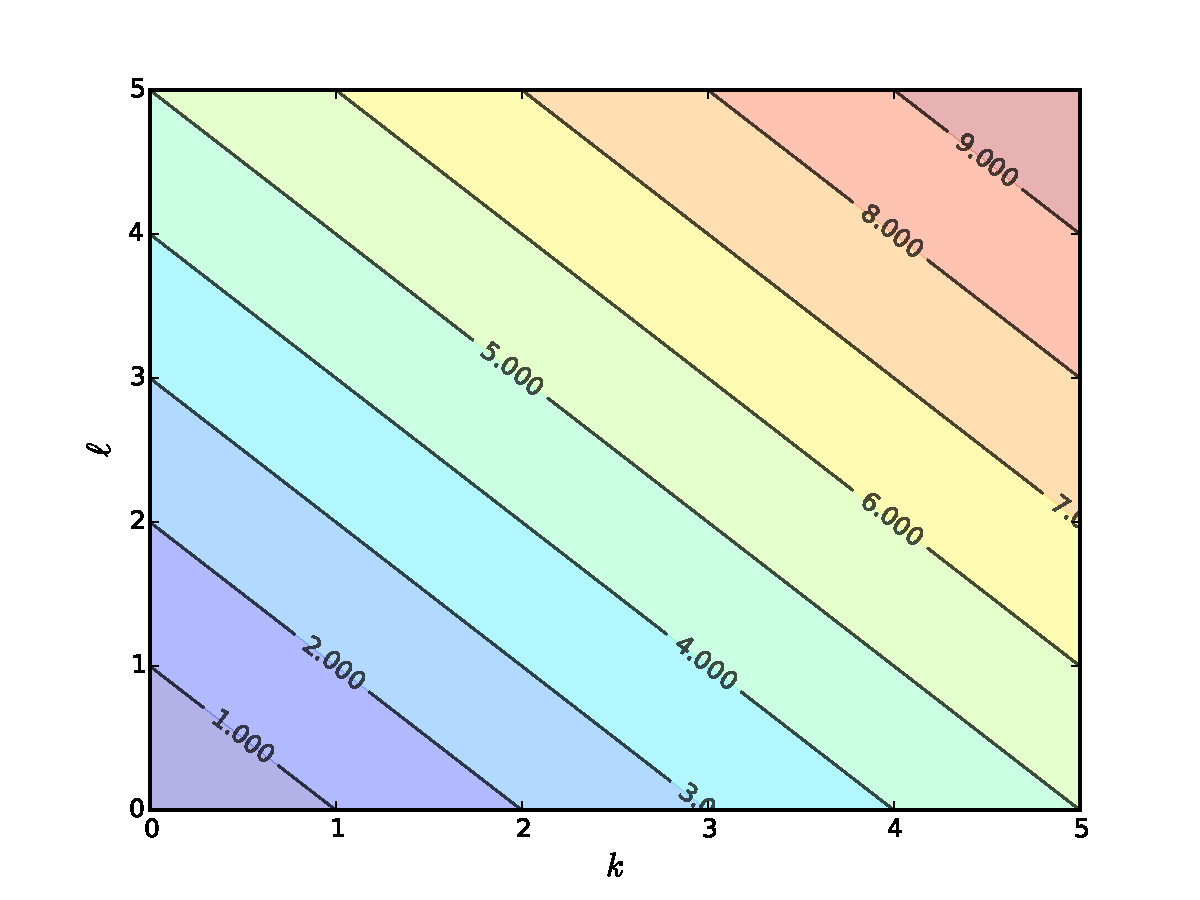
\includegraphics{cost_min_2.pdf}}
       \end{center}
    \end{figure}

   \Eg Cost function $c(k, \ell) = rk + w\ell$ cannot be one-to-one

\end{frame}

\begin{frame}\frametitle{Orthogonal Vectors and Projections}
    
    \vspace{2em}
    A core concept in the course is orthogonality -- not just of vectors,
     but random variables 
    
    \vspace{.7em}
    Let $\boldx$ and $\boldz$ be vectors in $\RR^N$
    
    If $\inner{\boldx,  \boldz} = 0$,
    then we  call $\boldx$ and $\boldz$
    \navy{orthogonal}
    
    Write \navy{$\boldx \perp \boldz$}
    
    In $\RR^2$, orthogonal means perpendicular 
    
\end{frame}

\begin{frame}

    \begin{figure}
       \begin{center}
        \begin{tikzpicture}[
    scale=5,
    axis/.style={<->, >=stealth'},
    important line/.style={thick},
    dotted line/.style={dotted, thick,red},
    every node/.style={color=black}
    ]

    % define x,z
    \coordinate(O) at (0,0);
    \coordinate (X) at (-0.2,0.3);
    \coordinate (Z) at (0.6,0.3);
    % axis
    \draw[axis] (-0.4,0)  -- (0.9,0) node(xline)[right] {};
    \draw[axis] (0,-0.3) -- (0,0.7) node(yline)[above] {};
    % x, z
    \draw[important line,blue, ->]  (O) -- (X) node[left] {$\boldx$};
    \draw[important line,blue, ->]  (O) -- (Z) node[right] {$\boldz$};
    % label angle
    \draw[dotted line] (-0.03,0.045) -- (0.03,0.075);
    \draw[dotted line] (0.06,0.03) -- (0.03,0.075);
\end{tikzpicture}

        \caption{\label{f:xpz} $\boldx \perp \boldz$}
       \end{center}
    \end{figure}

\end{frame}

\begin{frame}

     \vspace{2em}
    Let $S$ be a linear subspace
    
    \vspace{.7em}
    We say that 
    \navy{$\boldx$ is orthogonal to $S$} if $\boldx \perp \boldz$ for all 
    $\boldz \in S$

    Write \navy{$\boldx \perp S$}
    
\end{frame}


\begin{frame}
    
    \begin{figure}
       \begin{center}
        \begin{tikzpicture}[
    scale=5,
    axis/.style={<->, >=stealth'},
    important line/.style={thick},
    dotted line/.style={dotted, thick,red},
    every node/.style={color=black}
    ]

    % define x,z
    \coordinate(O) at (0,0);
    \coordinate (X) at (-0.2,0.3);
    \coordinate (Z1) at (-0.3,-0.15);
    \coordinate (Z2) at (0.8,0.4);
    % axis
    \draw[axis] (-0.4,0)  -- (0.9,0) node(xline)[right] {};
    \draw[axis] (0,-0.3) -- (0,0.7) node(yline)[above] {};
    % x, z
    \draw[important line,blue, ->]  (O) -- (X) node[left] {$\boldx$};
    \draw[important line]  (Z1) -- (Z2) node[right] {$S$};
    % label angle
    \draw[dotted line] (-0.03,0.045) -- (0.03,0.075);
    \draw[dotted line] (0.06,0.03) -- (0.03,0.075);
\end{tikzpicture}

        \caption{\label{f:xpS} $\boldx \perp S$}
       \end{center}
    \end{figure}

\end{frame}

\begin{frame}

    \vspace{2em}
    \Fact\eqref{ET-fa:pythag}
        (Pythagorian law)
        
        If $\{\boldz_1,\ldots, \boldz_K\}$ is an orthogonal set, then
        %
        \begin{equation*}
            \| \boldz_1 + \cdots + \boldz_K \|^2 
            = \| \boldz_1 \|^2 + \cdots + \| \boldz_K \|^2 
        \end{equation*}
        %
    Proof is an exercise 
    
    \vspace{.7em}
    \Fact\eqref{ET-fa:orthii}
    If $O \subset \RR^N$ is an orthogonal set and $\boldzero \notin O$, then
    $O$ is linearly independent
    
\end{frame}

\begin{frame}
    
    \vspace{2em}
    An orthogonal set $O \subset \RR^N$ is called an \navy{orthonormal set} 
    if $\|\boldu \| = 1$ for all $\boldu \in O$

    An orthonormal set spanning a linear
    subspace $S$ of $\RR^N$ is  an \navy{orthonormal basis} of $S$
    
    \begin{itemize}
        \item example of an orthonormal basis for all of $\RR^N$ is the canonical
        basis $\{\bolde_1, \ldots, \bolde_N\}$
    \end{itemize}
    
    \vspace{1em}
    \Fact\eqref{ET-fa:bdons}
    If $\{\boldu_1, \ldots, \boldu_K\}$ is an orthonormal set
    and $\boldx \in \Span\{\boldu_1, \ldots, \boldu_K\}$, then
    %
    \begin{equation*}
        \label{eq:exbyob}
        \boldx = \sum_{k=1}^K \inner{\boldx, \boldu_k} \boldu_k
    \end{equation*}
    %
\end{frame}

\section{Orthogonality}

\begin{frame}
    
    \vspace{2em}
    Given $S \subset \RR^N$, the \navy{orthogonal complement}
    of $S$ is
    %
    \begin{equation*}
        S^{\perp} := \setntn{\boldx \in \RR^N}{\boldx \perp S}
    \end{equation*}
    
    \vspace{.5em}
    \Fact\eqref{ET-fa:ocls}
    For any nonempty $S \subset \RR^N$, the set $S^{\perp}$ is
    a linear subspace of $\RR^N$
    
    \Prf 
    If $\boldx, \boldy \in S^{\perp}$ and $\alpha, \beta \in \RR$, then 
    $\alpha \boldx + \beta \boldy \in S^{\perp}$
    because, for any $\boldz \in S$
    %
    \begin{equation*}
        \inner{\alpha \boldx + \beta \boldy, \boldz}
         = \alpha \inner{ \boldx, \boldz} + \beta \inner{\boldy, \boldz}
         = \alpha \times 0  + \beta \times 0 
         = 0
    \end{equation*}
    
    \vspace{.5em}
    \Fact{\eqref{ET-fa:scscez}}
    For $S \subset \RR^N$, we have $S \cap S^{\perp} =
    \{\boldzero\}$
    
\end{frame}
   
\begin{frame}

    \vspace{2em}
    \begin{figure}
       \begin{center}
        \resizebox{7.5cm}{!}{\begin{tikzpicture}[
    scale=5,
    axis/.style={<->, >=stealth'},
    important line/.style={thick},
    dotted line/.style={dotted, thick,red},
    dashed line/.style={dashed, thin},
    every node/.style={color=black}
    ]

    % define x,z
    \coordinate(O) at (0,0);
    \coordinate (S1) at (-0.4,-0.2);
    \coordinate (S2) at (0.8,0.4);
    \coordinate (S3) at (-0.25,0.5);
    \coordinate (S4) at (0.12,-0.24); 
    % axis
    \draw[axis] (-0.5,0)  -- (0.9,0) node(xline)[right] {};
    \draw[axis] (0,-0.3) -- (0,0.7) node(yline)[above] {};
    % x, z
    \draw[important line, thick]  (S1) -- (S2) node[right] {$S$};
    \draw[important line, thick]  (S4) -- (S3) node[left] {$S^{\perp}$};
    % label angle
    \draw[dotted line] (-0.03,0.06) -- (0.03,0.09);
    \draw[dotted line] (0.06,0.03) -- (0.03,0.09);
   
\end{tikzpicture}
}
        \caption{\label{f:orth_comp} Orthogonal complement of $S$ in $\mathbb{R}^{2}$}
       \end{center}
    \end{figure}
    
\end{frame}

\begin{frame}\frametitle{The Orthogonal Projection Theorem}
    
    \vspace{2em}
    Problem:
    %
    \begin{center}
        Given $\boldy \in \RR^N$ and subspace $S$, find closest element of $S$ 
        to $\boldy$
    \end{center}
    
    Formally: Solve for
    %
    \begin{equation}\label{eq:mproj}
        \hboldy := \argmin_{\boldz \in S} \|\boldy - \boldz\|
    \end{equation}
    %
    Existence, uniqueness of solution not immediately obvious

    Orthogonal projection theorem: $\hboldy$ always exists, unique

    Also provides a useful characterization

\end{frame}

\begin{frame}
    
     \vspace{2em}
    \Thm\eqref{ET-t:opt}
    [Orthogonal Projection Theorem I]
    
    Let $\boldy \in \RR^N$ and let $S$ be any nonempty linear subspace of $\RR^N$. 
    
    The
    following statements are true:
    %
    \begin{enumerate}
        \item  The optimization problem \eqref{eq:mproj} has exactly one solution
        \item $\hboldy \in \RR^N$ solves \eqref{eq:mproj}
            if and only if $\hat \boldy \in S$ and $\boldy - \hat \boldy \perp
            S$
    \end{enumerate}
    
    \vspace{.7em}
    The unique solution $\hboldy$ is called the 
    \navy{orthogonal projection of $\boldy$ onto $S$}  

\end{frame}

\begin{frame}

    \vspace{2em}
    \begin{figure}
       \begin{center}
        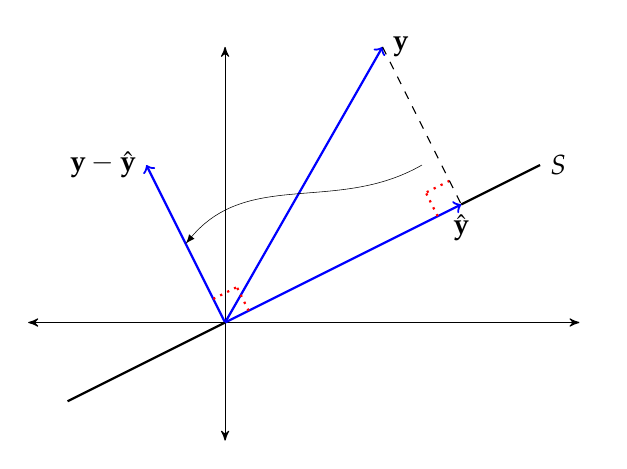
\begin{tikzpicture}[
    scale=5,
    axis/.style={<->, >=stealth'},
    important line/.style={thick},
    dotted line/.style={dotted, thick,red},
    dashed line/.style={dashed, thin},
    every node/.style={color=black}
    ]

    % define x,z
    \coordinate(O) at (0,0);
    \coordinate (y-yhat) at (-0.2,0.4);
    \coordinate (yhat) at (0.6,0.3);
    \coordinate (y) at (0.4,0.7);
    \coordinate (Z1) at (-0.4,-0.2);
    \coordinate (Z2) at (0.8,0.4);
    % axis
    \draw[axis] (-0.5,0)  -- (0.9,0) node(xline)[right] {};
    \draw[axis] (0,-0.3) -- (0,0.7) node(yline)[above] {};
    % x, z
    \draw[important line,blue,thick, ->]  (O) -- (yhat) node[below] {$\hboldy$};
    \draw[important line,blue, ->]  (O) -- (y-yhat) node[left] {$\boldy - \hboldy$};
    \draw[important line, thick]  (Z1) -- (O) node[right] {};
    \draw[important line, thick]  (yhat) -- (Z2) node[right] {$S$};
    \draw[important line, blue,->]  (O) -- (y) node[right] {$\boldy$};
    % label angle
    \draw[dotted line] (-0.03,0.06) -- (0.03,0.09);
    \draw[dotted line] (0.06,0.03) -- (0.03,0.09);
    \draw[dotted line] (0.54,0.27) -- (0.51,0.33);
    \draw[dotted line] (0.57,0.36) -- (0.51,0.33);
    \draw[dashed line, black] (y) -- (yhat);
    % path
    \draw[-latex, very thin] (0.5,0.4) to [out=210,in=50] (-0.1,0.2);
\end{tikzpicture}

        \caption{\label{f:orth_proj2D0} Orthogonal projection}
       \end{center}
    \end{figure}

\end{frame}

\begin{frame}

     \vspace{2em}
    \Prf (sufficiency of 2.)
    Let $\boldy \in \RR^N$
    and let $S$ be a linear subspace of $\RR^N$
    
    Let $\hat \boldy$ be a vector in
    $S$ satisfying $\boldy - \hat \boldy \perp S$
    
    Let $\boldz$ be any point in $S$. We have
    %
    \begin{equation*}
    \| \boldy - \boldz \|^2
    = \| (\boldy - \hat \boldy) + (\hat \boldy - \boldz) \|^2
    = \| \boldy - \hat \boldy \|^2  + \| \hat \boldy - \boldz  \|^2
    \end{equation*}
    %
    The second equality follows from $\boldy - \hat \boldy \perp S$ and the 
    Pythagorian law
    
    \vspace{.7em}
    Since $\boldz$ was an arbitrary point in $S$,
    we have $\| \boldy - \boldz \| \geq \| \boldy - \hat \boldy \|$
    for all $\boldz \in S$
    
\end{frame}

\begin{frame}

    \vspace{2em}
    \Eg
    Let $\boldy \in \RR^N$ and let $\boldone \in \RR^N$ be the vector of ones
    
    Let $S$ be the set of constant vectors in $\RR^N$--- $S$ is the span of $\{\boldone\}$
    
    Orthogonal projection of $\boldy$ onto $S$ is $\hboldy := \bar y
    \boldone$, where $\bar y := \frac{1}{N} \sum_{n=1}^N y_n$
    
    Clearly, $\hboldy \in S$ 
    
    \vspace{.7em}
    To show $\boldy -
    \hboldy$ is orthogonal to $S$, we need to check
    $\inner{\boldy - \hboldy, \boldone} = 0$ (see ex.~\ref{ET-ex:pecb} on
    page~\pageref{ET-ex:pecb}).  This is true because
    %
    \begin{equation*}
        \inner{\boldy - \hboldy, \boldone }
        = \inner{\boldy, \boldone} - \inner{\hboldy, \boldone}
        = \sum_{n=1}^N y_n - \bar y \inner{\boldone, \boldone}
        = 0
    \end{equation*}
    
\end{frame}

\begin{frame}
    
    \vspace{2em}
    Holding subspace $S$ fixed, we have a functional relationship
    %
    \begin{equation*}
        \boldy \; \mapsto \text{ its orthogonal projection } \hat \boldy \in S
    \end{equation*}
    %
    This is a well-defined function from $\RR^N$ to $\RR^N$
    
    \vspace{.7em}
    The function is typically denoted by $\boldP$

    \begin{itemize}
        \item $\boldP(\boldy)$ or $\boldP \boldy$ represents $\hboldy$
    \end{itemize}
    
    $\boldP$ is called the \navy{orthogonal projection mapping onto $S$} and we write
    %
    \begin{equation*}
        \boldP = \proj S
    \end{equation*}

\end{frame}

\begin{frame}

     \vspace{2em}
    \begin{figure}
       \begin{center}
        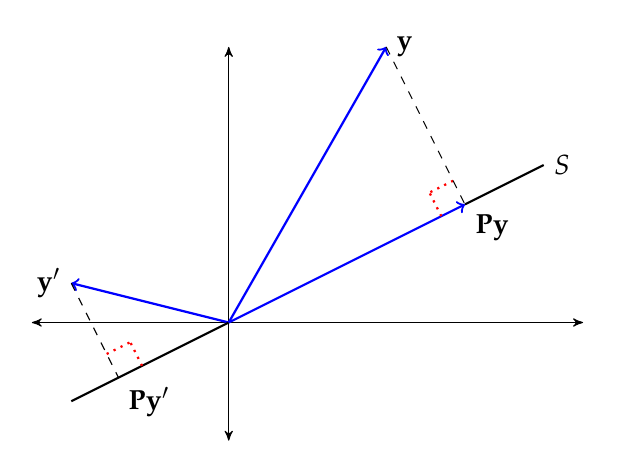
\begin{tikzpicture}[
    scale=5,
    axis/.style={<->, >=stealth'},
    important line/.style={thick},
    dotted line/.style={dotted, thick,red},
    dashed line/.style={dashed, thin},
    every node/.style={color=black}
    ]

    % define x,z
    \coordinate(O) at (0,0);
    \coordinate (y') at (-0.4,0.1);
    \coordinate (Py) at (0.6,0.3);
    \coordinate (y) at (0.4,0.7);
    \coordinate (Z1) at (-0.4,-0.2);
    \coordinate (Z2) at (0.8,0.4);
    \coordinate (Py') at (-0.28,-0.14);
    % axis
    \draw[axis] (-0.5,0)  -- (0.9,0) node(xline)[right] {};
    \draw[axis] (0,-0.3) -- (0,0.7) node(yline)[above] {};
    % x, z
    \draw[important line,blue,thick, ->]  (O) -- (Py) node[anchor = north west, text width=2em] {$\boldP \boldy$};
    \draw[important line,blue, ->]  (O) -- (y') node[left] {$\boldy'$};
    \draw[important line, thick]  (Z1) -- (O) node[right] {};
    \draw[important line, thick]  (Py) -- (Z2) node[right] {$S$};
    \draw[important line, blue,->]  (O) -- (y) node[right] {$\boldy$};
    % label angle
    \draw[dotted line] (0.54,0.27) -- (0.51,0.33);
    \draw[dotted line] (0.57,0.36) -- (0.51,0.33);
    \draw[dotted line] (-0.22,-0.11) -- (-0.25,-0.05);
    \draw[dotted line] (-0.31,-0.08) -- (-0.25,-0.05);
    \draw[dashed line, black] (y) -- (Py);
    \draw[dashed line, black] (y') -- (Py') node[anchor = north west, text width=5em] {$\boldP \boldy'$};
  
\end{tikzpicture}

        \caption{\label{f:orth_proj2Dp} Orthogonal projection under $\boldP$}
       \end{center}
    \end{figure}
    
\end{frame}

\begin{frame}

    \vspace{2em}
    \Thm{\eqref{ET-t:opt2}}
    [Orthogonal Projection Theorem II]
    Let $S$ be any linear subspace of $\RR^N$, and let $\boldP = \proj S$.
    The following statements are true:
    %
    \begin{enumerate}
        \item $\boldP$ is a linear function
    \end{enumerate}
    %
    Moreover, for any $\boldy \in \RR^N$, we have
    %
    \begin{enumerate}
        \setcounter{enumi}{1}
        \item $\boldP \boldy \in S$,
        \item $\boldy - \boldP \boldy \perp S$,
        \item $\| \boldy \|^2 = \| \boldP \boldy \|^2 + \| \boldy - \boldP
            \boldy \|^2$,
        \item $\| \boldP \boldy \| \leq \| \boldy \|$,
        \item $\boldP \boldy = \boldy$ if and only if $\boldy \in S$, and
        \item $\boldP \boldy = \boldzero$ if and only if $\boldy \in
            S^{\perp}$.
    \end{enumerate}
    %
    For a discussion of the proof, see page~\pageref{ET-t:opt2} and
     exercise \ref{ET-ex:prpil}
    
\end{frame}

\begin{frame}

     \vspace{2em}
    The following is a fundamental result 
    
    \vspace{.7em}
    \Fact{\eqref{ET-fa:projon}}
    If $\{\boldu_1, \ldots, \boldu_K\}$ is an orthonormal basis for $S$, then,
    for each $\boldy \in \RR^N$,
    %
    \begin{equation}
        \label{eq:projon}
        \boldP \boldy = \sum_{k=1}^K \inner{\boldy, \boldu_k} \boldu_k
    \end{equation}
    %
\end{frame}

\begin{frame}

     \vspace{2em}
    \Prf 
     First, the right-hand side of \eqref{eq:projon} lies in $S$ 
    since it is a linear combination of vectors spanning $S$
    
    Next, we know $\boldy - \boldP \boldy \perp S$ if and only if 
    $\boldy - \boldP \boldy \perp \boldu_j$ for each $\boldu_j$ in the 
    basis set (exercise ex.~\ref{ET-ex:pecb})
    
    For any $\boldy - \boldP \boldy \perp \boldu_j$, the following holds
    %
    \begin{multline*}
        \inner{\boldy - \boldP \boldy, \boldu_j}
        = \inner{\boldy, \boldu_j }
        -  \sum_{k=1}^K \inner{\boldy, \boldu_k} \inner{\boldu_k, \boldu_j}
        \\ = \inner{\boldy, \boldu_j} - \inner{\boldy, \boldu_j }
        = 0
    \end{multline*}
    %
    This confirms $\boldy - \boldP \boldy \perp S$ 
    
\end{frame}

\begin{frame}

     \vspace{2em}
    \Fact{\eqref{ET-fa:subsub}}
    Let $S_i$ be a linear subspace of $\RR^N$ for $i=1,2$ and let $\boldP_i =
    \proj S_i$.  If $S_1 \subset S_2$, then
    %
    \begin{equation*}
        \boldP_1 \boldP_2 \boldy = \boldP_2 \boldP_1 \boldy = \boldP_1 \boldy
        \quad \text{for all } \boldy \in \RR^N
    \end{equation*}
    %

\end{frame}

\begin{frame}\frametitle{The Residual Projection}

    \vspace{2em}
    Project $\boldy$ onto $S$, where $S$ is a linear subspace of $\RR^N$
    \begin{itemize}
    \item Closest point to $\boldy$ in $S$ is $\hboldy := \boldP \boldy$ 
		    here $\boldP = \proj S$
    \item Unless $\boldy$ was already in $S$, some error $\boldy -
    \boldP \boldy$ remains
    \end{itemize}
    
    \vspace{.7em}
    Introduce operator $\boldM$ that takes $\boldy \in \RR^N$
    and returns the residual
    \begin{equation}
        \label{eq:ann0}
        \boldM := \boldI - \boldP
    \end{equation}
    %
    where $\boldI$ is the identity mapping on $\RR^N$
    
\end{frame}

\begin{frame}

     \vspace{2em}
    For any $\boldy$ we have 
    $\boldM \boldy = \boldI \boldy - \boldP \boldy = \boldy - \boldP \boldy$
    
    \vspace{.7em}
    In regression analysis $\boldM$ shows up as a matrix 
    called the ``annihilator'
    
    \vspace{.7em}
    We  refer to $\boldM$ as the \navy{residual projection}
    
\end{frame}

\begin{frame}

     \vspace{2em}
    \Eg
    Recall the projection of
    $\boldy \in \RR^N$ onto $\Span\{\boldone\}$ is
    $\bar y \boldone$
    
    The residual projection is $\boldM_c \boldy := \boldy -
    \bar y \boldone$
    \begin{itemize}
        \item  vector of errors obtained when the elements of a vector are
         predicted by its sample mean
    \end{itemize}
    
    
\end{frame}

\begin{frame}

    \vspace{2em}
    \Fact{\eqref{ET-fa:opt3}}
    Let $S$ be a linear subspace of $\RR^N$, let $\boldP = \proj S$, and let
    $\boldM$ be the residual projection as defined in \eqref{eq:ann0}.  The
    following statements are true:
    %
    \begin{enumerate}
        \item $\boldM = \proj S^{\perp}$
        \item $\boldy = \boldP \boldy + \boldM \boldy$ for any $\boldy \in
            \RR^N$
        \item $\boldP \boldy \perp \boldM \boldy$ for any $\boldy \in \RR^N$
        \item $\boldM \boldy = \boldzero$ if and only if $\boldy \in S$
        \item $\boldP \circ \boldM = \boldM \circ \boldP = \boldzero$
    \end{enumerate}
    %
\end{frame}

\begin{frame}
    
    \vspace{2em}
    \begin{figure}
       \begin{center}
        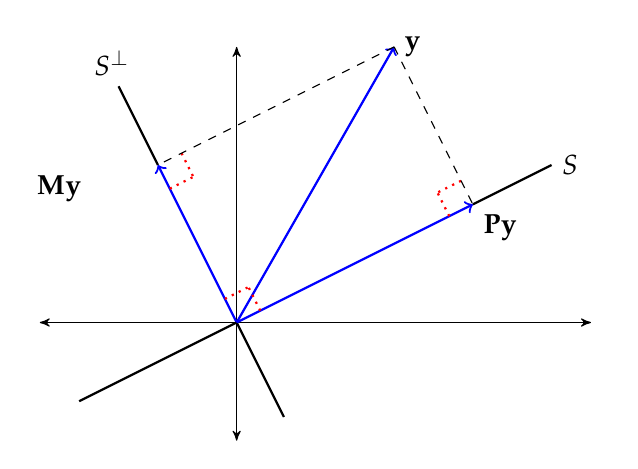
\begin{tikzpicture}[
    scale=5,
    axis/.style={<->, >=stealth'},
    important line/.style={thick},
    dotted line/.style={dotted, thick,red},
    dashed line/.style={dashed, thin},
    every node/.style={color=black}
    ]

    % define x,z
    \coordinate(O) at (0,0);
    \coordinate (uhat) at (-0.2,0.4);
    \coordinate (yhat) at (0.6,0.3);
    \coordinate (y) at (0.4,0.7);
    \coordinate (S1) at (-0.4,-0.2);
    \coordinate (S2) at (0.8,0.4);
    \coordinate (S3) at (-0.3,0.6);
    \coordinate (S4) at (0.12,-0.24); 
    % axis
    \draw[axis] (-0.5,0)  -- (0.9,0) node(xline)[right] {};
    \draw[axis] (0,-0.3) -- (0,0.7) node(yline)[above] {};
    % x, z
    \draw[important line,blue,thick, ->]  (O) -- (yhat) node[anchor = north west, text width=4em] {$\boldP \boldy$};
    \draw[important line,blue, ->]  (O) -- (uhat) node[anchor = north east, text width=4em] {$\boldM \boldy$};
    \draw[important line,thick] (uhat) -- (S3) node [anchor = south east, text width=0.5em] {$S^{\perp}$};
    \draw[important line,thick] (O) -- (S4);
    \draw[important line, thick]  (S1) -- (O) node[right] {};
    \draw[important line, thick]  (yhat) -- (S2) node[right] {$S$};
    \draw[important line, blue,->]  (O) -- (y) node[right] {$\boldy$};
    % label angle
    \draw[dotted line] (-0.03,0.06) -- (0.03,0.09);
    \draw[dotted line] (0.06,0.03) -- (0.03,0.09);
    \draw[dotted line] (0.54,0.27) -- (0.51,0.33);
    \draw[dotted line] (0.57,0.36) -- (0.51,0.33);
    \draw[dotted line] (-0.17,0.34) -- (-0.11,0.37);
    \draw[dotted line] (-0.14,0.43) -- (-0.11,0.37);
    
    \draw[dashed line, black] (y) -- (yhat);
    \draw[dashed line, black] (y) -- (uhat);
    
\end{tikzpicture}

        \caption{\label{f:orth_proj2D} The residual projection}
       \end{center}
    \end{figure}
    
\end{frame}


\begin{frame}

    \vspace{2em}
    If $S_1$ and $S_2$ are two subspaces of $\RR^N$ with $S_1 \subset S_2$, 
    then $S_2^{\perp} \subset S_1^{\perp}$

    The result in
    fact~\ref{ET-fa:subsub} is reversed for $\boldM$
    
    \vspace{.7em}
    \Fact{\eqref{ET-fa:subsub2}}
    Let $S_1$ and $S_2$ be two subspaces of $\RR^N$ and let 
    $\boldy \in \RR^N$.  Let $\boldM_1$ and $\boldM_2$ be the projections onto $S_1^{\perp}$
    and $S_2^{\perp}$ respectively.  If $S_1 \subset S_2$, then
    %
    \begin{equation*}
        \boldM_1 \boldM_2 \boldy = \boldM_2 \boldM_1 \boldy = \boldM_2 \boldy
    \end{equation*}
        
\end{frame}

\begin{frame}\frametitle{Gram-- Schmidt Orthogonalization} 

    \vspace{2em}
    Recall we showed every orthogonal subset of $\mathbb{R}^{N}$ not 
    containing $\textbf{0}$ is linearly independent -- fact~\ref{ET-fa:orthii}
    
    Here is an (important) partial converse 
    
    \vspace{.7em}
    \Thm{\eqref{ET-t:gso}}
    For each linearly independent set $\{\boldb_1, \ldots, \boldb_K\} \subset 
    \RR^N$, there exists an orthonormal set $\{\boldu_1, \ldots, \boldu_K\}$
    with
    %
    \begin{equation*}
        \Span \{\boldb_1, \ldots, \boldb_k\}
        = 
        \Span \{\boldu_1, \ldots, \boldu_k\}
        \quad \text{for } \;
        k = 1, \ldots, K
    \end{equation*}
    %
    Formal proofs are solved as exercises~\ref{ET-ex:gsso}~to~\ref{ET-ex:gssth}
    
\end{frame}


\begin{frame}
    
    \vspace{2em}
    The proof provides an important algorithm for generating
    the orthonormal set $\{\boldu_1, \ldots, \boldu_K\}$
    
    \vspace{1em}
    The first step is to
    construct orthogonal sets $\{\boldv_1, \ldots, \boldv_k\}$ with span identical
    to $\{\boldb_1, \ldots, \boldb_k\}$ for each $k$
    
    The construction of
    $\{\boldv_1, \ldots, \boldv_K\}$ uses the \navy{Gram--Schmidt
    orthogonalization} procedure:
    
    For each $k = 1, \ldots, K$, let 
    %
    \begin{enumerate}
        \item $B_k := \Span\{\boldb_1, \ldots, \boldb_k\}$,
        \item $\boldP_k := \proj B_k$ and $\boldM_k := \proj B_k^{\perp}$,
        \item $\boldv_k := \boldM_{k-1} \boldb_k$ where $\boldM_0$ is the identity
            mapping, and
        \item $V_k := \Span\{\boldv_1, \ldots, \boldv_k\}$.
    \end{enumerate}
    
\end{frame}

\begin{frame}

    \vspace{2em}
    In step 3. we map each successive element $\boldb_k$ into a subspace 
    orthogonal to the subspace generated by $\boldb_1, \ldots, \boldb_{k-1}$
    
    \vspace{.7em}
    To complete the argument, define $\boldu_k$ by $\boldu_k :=
    \boldv_k / \| \boldv_k \|$ 
    
    The  set of vectors 
    $\{\boldu_1, \ldots, \boldu_k\}$ is orthonormal with span equal to $V_k$
    
\end{frame}

\end{document}

